% Options for packages loaded elsewhere
\PassOptionsToPackage{unicode}{hyperref}
\PassOptionsToPackage{hyphens}{url}
\PassOptionsToPackage{dvipsnames,svgnames,x11names}{xcolor}
%
\documentclass[
  letterpaper,
  DIV=11,
  numbers=noendperiod]{scrreprt}

\usepackage{amsmath,amssymb}
\usepackage{iftex}
\ifPDFTeX
  \usepackage[T1]{fontenc}
  \usepackage[utf8]{inputenc}
  \usepackage{textcomp} % provide euro and other symbols
\else % if luatex or xetex
  \usepackage{unicode-math}
  \defaultfontfeatures{Scale=MatchLowercase}
  \defaultfontfeatures[\rmfamily]{Ligatures=TeX,Scale=1}
\fi
\usepackage{lmodern}
\ifPDFTeX\else  
    % xetex/luatex font selection
\fi
% Use upquote if available, for straight quotes in verbatim environments
\IfFileExists{upquote.sty}{\usepackage{upquote}}{}
\IfFileExists{microtype.sty}{% use microtype if available
  \usepackage[]{microtype}
  \UseMicrotypeSet[protrusion]{basicmath} % disable protrusion for tt fonts
}{}
\makeatletter
\@ifundefined{KOMAClassName}{% if non-KOMA class
  \IfFileExists{parskip.sty}{%
    \usepackage{parskip}
  }{% else
    \setlength{\parindent}{0pt}
    \setlength{\parskip}{6pt plus 2pt minus 1pt}}
}{% if KOMA class
  \KOMAoptions{parskip=half}}
\makeatother
\usepackage{xcolor}
\setlength{\emergencystretch}{3em} % prevent overfull lines
\setcounter{secnumdepth}{5}
% Make \paragraph and \subparagraph free-standing
\ifx\paragraph\undefined\else
  \let\oldparagraph\paragraph
  \renewcommand{\paragraph}[1]{\oldparagraph{#1}\mbox{}}
\fi
\ifx\subparagraph\undefined\else
  \let\oldsubparagraph\subparagraph
  \renewcommand{\subparagraph}[1]{\oldsubparagraph{#1}\mbox{}}
\fi

\usepackage{color}
\usepackage{fancyvrb}
\newcommand{\VerbBar}{|}
\newcommand{\VERB}{\Verb[commandchars=\\\{\}]}
\DefineVerbatimEnvironment{Highlighting}{Verbatim}{commandchars=\\\{\}}
% Add ',fontsize=\small' for more characters per line
\usepackage{framed}
\definecolor{shadecolor}{RGB}{241,243,245}
\newenvironment{Shaded}{\begin{snugshade}}{\end{snugshade}}
\newcommand{\AlertTok}[1]{\textcolor[rgb]{0.68,0.00,0.00}{#1}}
\newcommand{\AnnotationTok}[1]{\textcolor[rgb]{0.37,0.37,0.37}{#1}}
\newcommand{\AttributeTok}[1]{\textcolor[rgb]{0.40,0.45,0.13}{#1}}
\newcommand{\BaseNTok}[1]{\textcolor[rgb]{0.68,0.00,0.00}{#1}}
\newcommand{\BuiltInTok}[1]{\textcolor[rgb]{0.00,0.23,0.31}{#1}}
\newcommand{\CharTok}[1]{\textcolor[rgb]{0.13,0.47,0.30}{#1}}
\newcommand{\CommentTok}[1]{\textcolor[rgb]{0.37,0.37,0.37}{#1}}
\newcommand{\CommentVarTok}[1]{\textcolor[rgb]{0.37,0.37,0.37}{\textit{#1}}}
\newcommand{\ConstantTok}[1]{\textcolor[rgb]{0.56,0.35,0.01}{#1}}
\newcommand{\ControlFlowTok}[1]{\textcolor[rgb]{0.00,0.23,0.31}{#1}}
\newcommand{\DataTypeTok}[1]{\textcolor[rgb]{0.68,0.00,0.00}{#1}}
\newcommand{\DecValTok}[1]{\textcolor[rgb]{0.68,0.00,0.00}{#1}}
\newcommand{\DocumentationTok}[1]{\textcolor[rgb]{0.37,0.37,0.37}{\textit{#1}}}
\newcommand{\ErrorTok}[1]{\textcolor[rgb]{0.68,0.00,0.00}{#1}}
\newcommand{\ExtensionTok}[1]{\textcolor[rgb]{0.00,0.23,0.31}{#1}}
\newcommand{\FloatTok}[1]{\textcolor[rgb]{0.68,0.00,0.00}{#1}}
\newcommand{\FunctionTok}[1]{\textcolor[rgb]{0.28,0.35,0.67}{#1}}
\newcommand{\ImportTok}[1]{\textcolor[rgb]{0.00,0.46,0.62}{#1}}
\newcommand{\InformationTok}[1]{\textcolor[rgb]{0.37,0.37,0.37}{#1}}
\newcommand{\KeywordTok}[1]{\textcolor[rgb]{0.00,0.23,0.31}{#1}}
\newcommand{\NormalTok}[1]{\textcolor[rgb]{0.00,0.23,0.31}{#1}}
\newcommand{\OperatorTok}[1]{\textcolor[rgb]{0.37,0.37,0.37}{#1}}
\newcommand{\OtherTok}[1]{\textcolor[rgb]{0.00,0.23,0.31}{#1}}
\newcommand{\PreprocessorTok}[1]{\textcolor[rgb]{0.68,0.00,0.00}{#1}}
\newcommand{\RegionMarkerTok}[1]{\textcolor[rgb]{0.00,0.23,0.31}{#1}}
\newcommand{\SpecialCharTok}[1]{\textcolor[rgb]{0.37,0.37,0.37}{#1}}
\newcommand{\SpecialStringTok}[1]{\textcolor[rgb]{0.13,0.47,0.30}{#1}}
\newcommand{\StringTok}[1]{\textcolor[rgb]{0.13,0.47,0.30}{#1}}
\newcommand{\VariableTok}[1]{\textcolor[rgb]{0.07,0.07,0.07}{#1}}
\newcommand{\VerbatimStringTok}[1]{\textcolor[rgb]{0.13,0.47,0.30}{#1}}
\newcommand{\WarningTok}[1]{\textcolor[rgb]{0.37,0.37,0.37}{\textit{#1}}}

\providecommand{\tightlist}{%
  \setlength{\itemsep}{0pt}\setlength{\parskip}{0pt}}\usepackage{longtable,booktabs,array}
\usepackage{calc} % for calculating minipage widths
% Correct order of tables after \paragraph or \subparagraph
\usepackage{etoolbox}
\makeatletter
\patchcmd\longtable{\par}{\if@noskipsec\mbox{}\fi\par}{}{}
\makeatother
% Allow footnotes in longtable head/foot
\IfFileExists{footnotehyper.sty}{\usepackage{footnotehyper}}{\usepackage{footnote}}
\makesavenoteenv{longtable}
\usepackage{graphicx}
\makeatletter
\def\maxwidth{\ifdim\Gin@nat@width>\linewidth\linewidth\else\Gin@nat@width\fi}
\def\maxheight{\ifdim\Gin@nat@height>\textheight\textheight\else\Gin@nat@height\fi}
\makeatother
% Scale images if necessary, so that they will not overflow the page
% margins by default, and it is still possible to overwrite the defaults
% using explicit options in \includegraphics[width, height, ...]{}
\setkeys{Gin}{width=\maxwidth,height=\maxheight,keepaspectratio}
% Set default figure placement to htbp
\makeatletter
\def\fps@figure{htbp}
\makeatother

\KOMAoption{captions}{tableheading}
\makeatletter
\@ifpackageloaded{bookmark}{}{\usepackage{bookmark}}
\makeatother
\makeatletter
\@ifpackageloaded{caption}{}{\usepackage{caption}}
\AtBeginDocument{%
\ifdefined\contentsname
  \renewcommand*\contentsname{Table of contents}
\else
  \newcommand\contentsname{Table of contents}
\fi
\ifdefined\listfigurename
  \renewcommand*\listfigurename{List of Figures}
\else
  \newcommand\listfigurename{List of Figures}
\fi
\ifdefined\listtablename
  \renewcommand*\listtablename{List of Tables}
\else
  \newcommand\listtablename{List of Tables}
\fi
\ifdefined\figurename
  \renewcommand*\figurename{Figure}
\else
  \newcommand\figurename{Figure}
\fi
\ifdefined\tablename
  \renewcommand*\tablename{Table}
\else
  \newcommand\tablename{Table}
\fi
}
\@ifpackageloaded{float}{}{\usepackage{float}}
\floatstyle{ruled}
\@ifundefined{c@chapter}{\newfloat{codelisting}{h}{lop}}{\newfloat{codelisting}{h}{lop}[chapter]}
\floatname{codelisting}{Listing}
\newcommand*\listoflistings{\listof{codelisting}{List of Listings}}
\makeatother
\makeatletter
\makeatother
\makeatletter
\@ifpackageloaded{caption}{}{\usepackage{caption}}
\@ifpackageloaded{subcaption}{}{\usepackage{subcaption}}
\makeatother
\ifLuaTeX
  \usepackage{selnolig}  % disable illegal ligatures
\fi
\usepackage{bookmark}

\IfFileExists{xurl.sty}{\usepackage{xurl}}{} % add URL line breaks if available
\urlstyle{same} % disable monospaced font for URLs
\hypersetup{
  pdftitle={Notebooks},
  colorlinks=true,
  linkcolor={blue},
  filecolor={Maroon},
  citecolor={Blue},
  urlcolor={Blue},
  pdfcreator={LaTeX via pandoc}}

\title{Notebooks}
\author{}
\date{}

\begin{document}
\maketitle

\renewcommand*\contentsname{Table of contents}
{
\hypersetup{linkcolor=}
\setcounter{tocdepth}{2}
\tableofcontents
}
\bookmarksetup{startatroot}

\chapter{Index}\label{index}

This \href{https://quarto.org/docs/websites}{Quarto website} hosts my
notes for some of the programming/scripting languages that I have
learned.

\part{R}

\chapter{R Basics}\label{r-basics}

\section{General Notes}\label{general-notes}

\begin{itemize}
\tightlist
\item
  Creating a project instead of a file comes with the advantage of
  saving the workspace settings
\item
  An R package usually includes (a) reusable functions, (b)
  documentation describing how to use the function, and (c) sample data
\item
  \texttt{Ctrl+Enter}: run line on which cursor is standing
\item
  \texttt{Ctrl+Alt+I}: insert new code chunk
\item
  \texttt{Ctrl+Shift+C}: comment/un-comment
\end{itemize}

\section{Clear Workspace}\label{clear-workspace}

Start by cleaning the workspace environment of the project to avoid
mixing up variables created in other files.

\begin{Shaded}
\begin{Highlighting}[]
\FunctionTok{rm}\NormalTok{(}\AttributeTok{list=}\FunctionTok{ls}\NormalTok{())}
\end{Highlighting}
\end{Shaded}

\section{Data Types}\label{data-types}

\begin{itemize}
\tightlist
\item
  character
\item
  numeric
\item
  logical
\item
  raw
\item
  imaginary numbers
\end{itemize}

\begin{Shaded}
\begin{Highlighting}[]
\FunctionTok{class}\NormalTok{(x)    }\CommentTok{\# give the data type of x}
\end{Highlighting}
\end{Shaded}

\subsection{Mixing Data Types}\label{mixing-data-types}

\begin{itemize}
\tightlist
\item
  character + numeric --\textgreater{} character
\item
  numeric + logical --\textgreater{} numeric
\item
  numeric + character + logical --\textgreater{} character
\end{itemize}

\section{Data Structures}\label{data-structures}

\begin{itemize}
\tightlist
\item
  \textbf{vector}: hold single type of data
\item
  \textbf{matrix}: 2D vector
\item
  \textbf{array}: nD vector
\item
  \textbf{list}: generic vector, can hold mixed type of data, eg, one
  element can a character, another a list of integers, and the third
  could be a logical
\item
  \textbf{data frame}: table where columns represent vectors
\item
  \textbf{tibbles}: data frames, but slightly tweaked to work better
  with \texttt{tidyverse} package
\item
  \textbf{factor}
\end{itemize}

\begin{figure}

\centering{

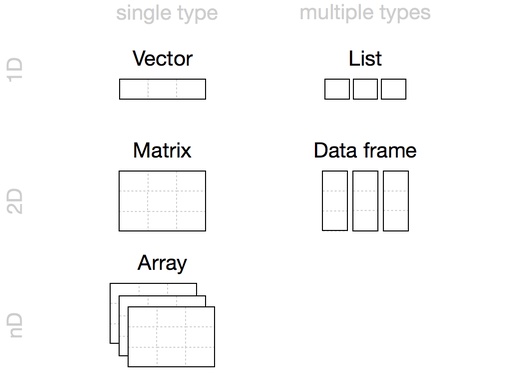
\includegraphics[width=1.71in,height=\textheight]{src/../images/datastructure.png}

}

\caption{\label{fig-datastructure}Common data structures in R (Source:
\href{https://jjallaire.github.io/hopr/objects.html}{Grolemund, 2014})}

\end{figure}%

\begin{Shaded}
\begin{Highlighting}[]
\FunctionTok{str}\NormalTok{(x)      }\CommentTok{\# give the structure type of x}
\FunctionTok{length}\NormalTok{(x)   }\CommentTok{\# length of structure}
\end{Highlighting}
\end{Shaded}

\section{Basics Operations}\label{basics-operations}

Assignment

\begin{Shaded}
\begin{Highlighting}[]
\NormalTok{x }\OtherTok{\textless{}{-}} \DecValTok{3}      \CommentTok{\# assign 3 to x}
\NormalTok{(x }\OtherTok{\textless{}{-}} \DecValTok{3}\NormalTok{)    }\CommentTok{\# assign 3 to x \& print the result to console}
\end{Highlighting}
\end{Shaded}

\begin{verbatim}
[1] 3
\end{verbatim}

Getting Help

\begin{Shaded}
\begin{Highlighting}[]
\FunctionTok{args}\NormalTok{(round) }\CommentTok{\# print the argument list of function}
\NormalTok{?round        }\CommentTok{\# show documentation of function in Help window}
\end{Highlighting}
\end{Shaded}

Dealing with Structure

\begin{Shaded}
\begin{Highlighting}[]
\CommentTok{\# concatenate set of values to create vector}
\NormalTok{weight\_g }\OtherTok{\textless{}{-}} \FunctionTok{c}\NormalTok{(}\DecValTok{50}\NormalTok{, }\DecValTok{60}\NormalTok{, }\DecValTok{3}\NormalTok{, }\DecValTok{9}\NormalTok{)}
\NormalTok{animals }\OtherTok{\textless{}{-}} \FunctionTok{c}\NormalTok{(}\StringTok{"dog"}\NormalTok{, }\StringTok{"bat"}\NormalTok{, }\StringTok{"cat"}\NormalTok{)}

\CommentTok{\# utilizing logical values to pull specific values}
\NormalTok{weight\_g[weight\_g }\SpecialCharTok{\textless{}} \DecValTok{10} \SpecialCharTok{\&}\NormalTok{ weight\_g }\SpecialCharTok{\textgreater{}} \DecValTok{60} \SpecialCharTok{|}\NormalTok{ weight\_g }\SpecialCharTok{==} \DecValTok{50}\NormalTok{]}
\end{Highlighting}
\end{Shaded}

\begin{verbatim}
[1] 50
\end{verbatim}

\begin{Shaded}
\begin{Highlighting}[]
\CommentTok{\# pull dog \& cat records}
\NormalTok{animals[animals }\SpecialCharTok{\%in\%} \FunctionTok{c}\NormalTok{(}\StringTok{"dog"}\NormalTok{, }\StringTok{"cat"}\NormalTok{)]}
\end{Highlighting}
\end{Shaded}

\begin{verbatim}
[1] "dog" "cat"
\end{verbatim}

\begin{Shaded}
\begin{Highlighting}[]
\NormalTok{animals[animals }\SpecialCharTok{==} \StringTok{"dog"} \SpecialCharTok{|}\NormalTok{ animals }\SpecialCharTok{==} \StringTok{"cat"}\NormalTok{]}
\end{Highlighting}
\end{Shaded}

\begin{verbatim}
[1] "dog" "cat"
\end{verbatim}

Statistics

\begin{Shaded}
\begin{Highlighting}[]
\CommentTok{\# signaling missing data using NA}
\NormalTok{heights }\OtherTok{\textless{}{-}} \FunctionTok{c}\NormalTok{(}\DecValTok{2}\NormalTok{, }\DecValTok{3}\NormalTok{, }\ConstantTok{NA}\NormalTok{, }\DecValTok{4}\NormalTok{)}

\CommentTok{\# get mean while ignoring missing data}
\FunctionTok{mean}\NormalTok{(heights, }\AttributeTok{na.rm =} \ConstantTok{TRUE}\NormalTok{)}
\end{Highlighting}
\end{Shaded}

\begin{verbatim}
[1] 3
\end{verbatim}

\begin{Shaded}
\begin{Highlighting}[]
\CommentTok{\# how to use mean}
\CommentTok{\# ?mean}
\end{Highlighting}
\end{Shaded}

\section{Exploratory Operations}\label{exploratory-operations}

The \texttt{here} package makes it easy to point to files starting from
the project main directory.

\begin{Shaded}
\begin{Highlighting}[]
\FunctionTok{library}\NormalTok{(here)}
\end{Highlighting}
\end{Shaded}

Loading file from repository and saving it locally on disk. It is always
a good idea to structure the workspace--for more information, see
\href{http://journals.plos.org/plosbiology/article?id=10.1371/journal.pbio.1001745}{Best
Practices for Scientific Computing paper}.

\begin{Shaded}
\begin{Highlighting}[]
\FunctionTok{download.file}\NormalTok{(}\AttributeTok{url =} \StringTok{"https://ndownloader.figshare.com/files/2292169"}\NormalTok{, }
    \AttributeTok{destfile =} \FunctionTok{here}\NormalTok{(}\StringTok{"data"}\NormalTok{, }\StringTok{"portal\_data\_joined.csv"}\NormalTok{))}
\end{Highlighting}
\end{Shaded}

Load file to R as data frame

\begin{Shaded}
\begin{Highlighting}[]
\NormalTok{surveys }\OtherTok{\textless{}{-}} \FunctionTok{read.csv}\NormalTok{(}\FunctionTok{here}\NormalTok{(}\StringTok{"data"}\NormalTok{, }\StringTok{"portal\_data\_joined.csv"}\NormalTok{))}
\end{Highlighting}
\end{Shaded}

Inspecting data frame

\begin{Shaded}
\begin{Highlighting}[]
\FunctionTok{class}\NormalTok{(surveys)  }\CommentTok{\# data type}
\end{Highlighting}
\end{Shaded}

\begin{verbatim}
[1] "data.frame"
\end{verbatim}

\begin{Shaded}
\begin{Highlighting}[]
\FunctionTok{str}\NormalTok{(surveys)      }\CommentTok{\# structure}
\end{Highlighting}
\end{Shaded}

\begin{verbatim}
'data.frame':   34786 obs. of  13 variables:
 $ record_id      : int  1 72 224 266 349 363 435 506 588 661 ...
 $ month          : int  7 8 9 10 11 11 12 1 2 3 ...
 $ day            : int  16 19 13 16 12 12 10 8 18 11 ...
 $ year           : int  1977 1977 1977 1977 1977 1977 1977 1978 1978 1978 ...
 $ plot_id        : int  2 2 2 2 2 2 2 2 2 2 ...
 $ species_id     : chr  "NL" "NL" "NL" "NL" ...
 $ sex            : chr  "M" "M" "" "" ...
 $ hindfoot_length: int  32 31 NA NA NA NA NA NA NA NA ...
 $ weight         : int  NA NA NA NA NA NA NA NA 218 NA ...
 $ genus          : chr  "Neotoma" "Neotoma" "Neotoma" "Neotoma" ...
 $ species        : chr  "albigula" "albigula" "albigula" "albigula" ...
 $ taxa           : chr  "Rodent" "Rodent" "Rodent" "Rodent" ...
 $ plot_type      : chr  "Control" "Control" "Control" "Control" ...
\end{verbatim}

\begin{Shaded}
\begin{Highlighting}[]
\FunctionTok{dim}\NormalTok{(surveys)      }\CommentTok{\# dimensions}
\end{Highlighting}
\end{Shaded}

\begin{verbatim}
[1] 34786    13
\end{verbatim}

\begin{Shaded}
\begin{Highlighting}[]
\FunctionTok{nrow}\NormalTok{(surveys)}
\end{Highlighting}
\end{Shaded}

\begin{verbatim}
[1] 34786
\end{verbatim}

\begin{Shaded}
\begin{Highlighting}[]
\FunctionTok{ncol}\NormalTok{(surveys)}
\end{Highlighting}
\end{Shaded}

\begin{verbatim}
[1] 13
\end{verbatim}

\begin{Shaded}
\begin{Highlighting}[]
\FunctionTok{summary}\NormalTok{(surveys)}
\end{Highlighting}
\end{Shaded}

\begin{verbatim}
   record_id         month             day            year         plot_id     
 Min.   :    1   Min.   : 1.000   Min.   : 1.0   Min.   :1977   Min.   : 1.00  
 1st Qu.: 8964   1st Qu.: 4.000   1st Qu.: 9.0   1st Qu.:1984   1st Qu.: 5.00  
 Median :17762   Median : 6.000   Median :16.0   Median :1990   Median :11.00  
 Mean   :17804   Mean   : 6.474   Mean   :16.1   Mean   :1990   Mean   :11.34  
 3rd Qu.:26655   3rd Qu.:10.000   3rd Qu.:23.0   3rd Qu.:1997   3rd Qu.:17.00  
 Max.   :35548   Max.   :12.000   Max.   :31.0   Max.   :2002   Max.   :24.00  
                                                                               
  species_id            sex            hindfoot_length     weight      
 Length:34786       Length:34786       Min.   : 2.00   Min.   :  4.00  
 Class :character   Class :character   1st Qu.:21.00   1st Qu.: 20.00  
 Mode  :character   Mode  :character   Median :32.00   Median : 37.00  
                                       Mean   :29.29   Mean   : 42.67  
                                       3rd Qu.:36.00   3rd Qu.: 48.00  
                                       Max.   :70.00   Max.   :280.00  
                                       NA's   :3348    NA's   :2503    
    genus             species              taxa            plot_type        
 Length:34786       Length:34786       Length:34786       Length:34786      
 Class :character   Class :character   Class :character   Class :character  
 Mode  :character   Mode  :character   Mode  :character   Mode  :character  
                                                                            
                                                                            
                                                                            
                                                                            
\end{verbatim}

Show first/last few objects/records/rows

\begin{Shaded}
\begin{Highlighting}[]
\FunctionTok{head}\NormalTok{(surveys)}
\end{Highlighting}
\end{Shaded}

\begin{verbatim}
  record_id month day year plot_id species_id sex hindfoot_length weight
1         1     7  16 1977       2         NL   M              32     NA
2        72     8  19 1977       2         NL   M              31     NA
3       224     9  13 1977       2         NL                  NA     NA
4       266    10  16 1977       2         NL                  NA     NA
5       349    11  12 1977       2         NL                  NA     NA
6       363    11  12 1977       2         NL                  NA     NA
    genus  species   taxa plot_type
1 Neotoma albigula Rodent   Control
2 Neotoma albigula Rodent   Control
3 Neotoma albigula Rodent   Control
4 Neotoma albigula Rodent   Control
5 Neotoma albigula Rodent   Control
6 Neotoma albigula Rodent   Control
\end{verbatim}

\begin{Shaded}
\begin{Highlighting}[]
\FunctionTok{tail}\NormalTok{(surveys)}
\end{Highlighting}
\end{Shaded}

\begin{verbatim}
      record_id month day year plot_id species_id sex hindfoot_length weight
34781     26787     9  27 1997       7         PL   F              21     16
34782     26966    10  25 1997       7         PL   M              20     16
34783     27185    11  22 1997       7         PL   F              21     22
34784     27792     5   2 1998       7         PL   F              20      8
34785     28806    11  21 1998       7         PX                  NA     NA
34786     30986     7   1 2000       7         PX                  NA     NA
            genus  species   taxa        plot_type
34781  Peromyscus leucopus Rodent Rodent Exclosure
34782  Peromyscus leucopus Rodent Rodent Exclosure
34783  Peromyscus leucopus Rodent Rodent Exclosure
34784  Peromyscus leucopus Rodent Rodent Exclosure
34785 Chaetodipus      sp. Rodent Rodent Exclosure
34786 Chaetodipus      sp. Rodent Rodent Exclosure
\end{verbatim}

\subsection{Retrieve specific
element/row/column}\label{retrieve-specific-elementrowcolumn}

\begin{Shaded}
\begin{Highlighting}[]
\NormalTok{surveys[}\DecValTok{1}\NormalTok{,}\DecValTok{1}\NormalTok{]    }\CommentTok{\# element[1,1]}
\end{Highlighting}
\end{Shaded}

\begin{verbatim}
[1] 1
\end{verbatim}

\begin{Shaded}
\begin{Highlighting}[]
\NormalTok{surveys[}\DecValTok{1}\NormalTok{, ]    }\CommentTok{\# row 1}
\end{Highlighting}
\end{Shaded}

\begin{verbatim}
  record_id month day year plot_id species_id sex hindfoot_length weight
1         1     7  16 1977       2         NL   M              32     NA
    genus  species   taxa plot_type
1 Neotoma albigula Rodent   Control
\end{verbatim}

\begin{Shaded}
\begin{Highlighting}[]
\FunctionTok{head}\NormalTok{(surveys[ ,}\DecValTok{1}\NormalTok{])  }\CommentTok{\# column 1}
\end{Highlighting}
\end{Shaded}

\begin{verbatim}
[1]   1  72 224 266 349 363
\end{verbatim}

\begin{Shaded}
\begin{Highlighting}[]
\FunctionTok{head}\NormalTok{(surveys}\SpecialCharTok{$}\NormalTok{sex)     }\CommentTok{\# column by name}
\end{Highlighting}
\end{Shaded}

\begin{verbatim}
[1] "M" "M" ""  ""  ""  "" 
\end{verbatim}

\subsection{Dealing with factor (categorical)
columns}\label{dealing-with-factor-categorical-columns}

R convert columns that contain characters to factors by default. Factors
are treated as integer vectors. By default, R sorts levels in
alphabetical order.

\begin{Shaded}
\begin{Highlighting}[]
\FunctionTok{levels}\NormalTok{(surveys}\SpecialCharTok{$}\NormalTok{sex)}
\end{Highlighting}
\end{Shaded}

\begin{verbatim}
NULL
\end{verbatim}

\begin{Shaded}
\begin{Highlighting}[]
\FunctionTok{nlevels}\NormalTok{(surveys}\SpecialCharTok{$}\NormalTok{sex)}
\end{Highlighting}
\end{Shaded}

\begin{verbatim}
[1] 0
\end{verbatim}

Reorder factors (to get better plots)

\begin{Shaded}
\begin{Highlighting}[]
\NormalTok{surveys}\SpecialCharTok{$}\NormalTok{sex\_ordered }\OtherTok{\textless{}{-}} \FunctionTok{factor}\NormalTok{(surveys}\SpecialCharTok{$}\NormalTok{sex, }\AttributeTok{level=}\FunctionTok{c}\NormalTok{(}\StringTok{"F"}\NormalTok{, }\StringTok{"M"}\NormalTok{, }\StringTok{""}\NormalTok{))}
\FunctionTok{str}\NormalTok{(surveys}\SpecialCharTok{$}\NormalTok{sex\_ordered)}
\end{Highlighting}
\end{Shaded}

\begin{verbatim}
 Factor w/ 3 levels "F","M","": 2 2 3 3 3 3 3 3 2 3 ...
\end{verbatim}

\begin{Shaded}
\begin{Highlighting}[]
\FunctionTok{levels}\NormalTok{(surveys}\SpecialCharTok{$}\NormalTok{sex\_ordered)}
\end{Highlighting}
\end{Shaded}

\begin{verbatim}
[1] "F" "M" "" 
\end{verbatim}

\begin{Shaded}
\begin{Highlighting}[]
\FunctionTok{nlevels}\NormalTok{(surveys}\SpecialCharTok{$}\NormalTok{sex\_ordered)}
\end{Highlighting}
\end{Shaded}

\begin{verbatim}
[1] 3
\end{verbatim}

\subsection{Basic Plotting}\label{basic-plotting}

Histogram

\begin{Shaded}
\begin{Highlighting}[]
\CommentTok{\# plot(surveys$sex)  \# not possible}
\FunctionTok{plot}\NormalTok{(surveys}\SpecialCharTok{$}\NormalTok{sex\_ordered)}
\end{Highlighting}
\end{Shaded}

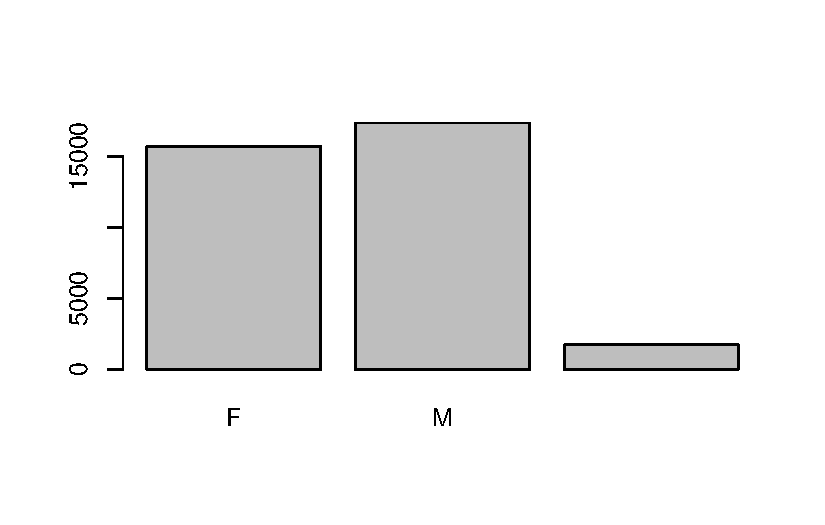
\includegraphics{src/r-basics_files/figure-pdf/unnamed-chunk-21-1.pdf}

Enhance the plot

\begin{Shaded}
\begin{Highlighting}[]
\FunctionTok{levels}\NormalTok{(surveys}\SpecialCharTok{$}\NormalTok{sex\_ordered)[}\DecValTok{1}\NormalTok{] }\OtherTok{\textless{}{-}} \StringTok{"Female"}
\FunctionTok{levels}\NormalTok{(surveys}\SpecialCharTok{$}\NormalTok{sex\_ordered)[}\DecValTok{2}\NormalTok{] }\OtherTok{\textless{}{-}} \StringTok{"Male"}
\FunctionTok{plot}\NormalTok{(surveys}\SpecialCharTok{$}\NormalTok{sex\_ordered)}
\end{Highlighting}
\end{Shaded}

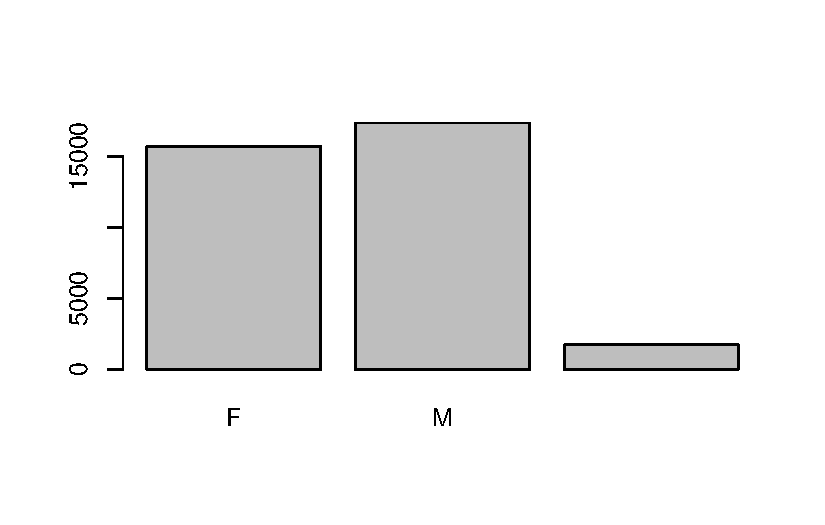
\includegraphics{src/r-basics_files/figure-pdf/unnamed-chunk-22-1.pdf}

\section{Data Manipulation}\label{data-manipulation}

\begin{itemize}
\tightlist
\item
  \texttt{tdlyr}

  \begin{itemize}
  \tightlist
  \item
    makes manipulation of data easier
  \item
    built to work with data frames directly
  \item
    can directly work with data stored in an external database which
    give the advantage of only bringing what we need to the memory to
    work on without having to bring the whole database
  \end{itemize}
\item
  \texttt{tidyr}

  \begin{itemize}
  \tightlist
  \item
    allows to swiftly convert b/w different data formats for plotting \&
    analysis in order to accommodate the different requirements by
    different functions

    \begin{itemize}
    \tightlist
    \item
      sometime we want one row per measurement
    \item
      other times we want the data aggregated like when plotting
    \end{itemize}
  \end{itemize}
\end{itemize}

Before using \texttt{tdlyr} and \texttt{tidyr}:

\begin{itemize}
\tightlist
\item
  Install \texttt{tidyverse} package: umbrella-package that install
  several packages (tidyr, dplyr, ggplot2 tibble, magrittr, etc.)
\item
  Load the package each session
\end{itemize}

Load packages

\begin{Shaded}
\begin{Highlighting}[]
\FunctionTok{library}\NormalTok{(}\StringTok{"tidyverse"}\NormalTok{)}
\end{Highlighting}
\end{Shaded}

\begin{verbatim}
-- Attaching core tidyverse packages ------------------------ tidyverse 2.0.0 --
v dplyr     1.1.4     v readr     2.1.5
v forcats   1.0.0     v stringr   1.5.1
v ggplot2   3.5.1     v tibble    3.2.1
v lubridate 1.9.3     v tidyr     1.3.1
v purrr     1.0.2     
-- Conflicts ------------------------------------------ tidyverse_conflicts() --
x dplyr::filter() masks stats::filter()
x dplyr::lag()    masks stats::lag()
i Use the conflicted package (<http://conflicted.r-lib.org/>) to force all conflicts to become errors
\end{verbatim}

Load \& inspect data

\begin{Shaded}
\begin{Highlighting}[]
\CommentTok{\# notice the \textquotesingle{}\_\textquotesingle{} instead of \textquotesingle{}.\textquotesingle{} of basic R}
\NormalTok{surveys }\OtherTok{\textless{}{-}} \FunctionTok{read\_csv}\NormalTok{(}\FunctionTok{here}\NormalTok{(}\StringTok{"data"}\NormalTok{, }\StringTok{"portal\_data\_joined.csv"}\NormalTok{))}
\end{Highlighting}
\end{Shaded}

\begin{verbatim}
Rows: 34786 Columns: 13
-- Column specification --------------------------------------------------------
Delimiter: ","
chr (6): species_id, sex, genus, species, taxa, plot_type
dbl (7): record_id, month, day, year, plot_id, hindfoot_length, weight

i Use `spec()` to retrieve the full column specification for this data.
i Specify the column types or set `show_col_types = FALSE` to quiet this message.
\end{verbatim}

\begin{Shaded}
\begin{Highlighting}[]
\FunctionTok{str}\NormalTok{(surveys)    }\CommentTok{\# structure: tbl\_df (tibble)}
\end{Highlighting}
\end{Shaded}

\begin{verbatim}
spc_tbl_ [34,786 x 13] (S3: spec_tbl_df/tbl_df/tbl/data.frame)
 $ record_id      : num [1:34786] 1 72 224 266 349 363 435 506 588 661 ...
 $ month          : num [1:34786] 7 8 9 10 11 11 12 1 2 3 ...
 $ day            : num [1:34786] 16 19 13 16 12 12 10 8 18 11 ...
 $ year           : num [1:34786] 1977 1977 1977 1977 1977 ...
 $ plot_id        : num [1:34786] 2 2 2 2 2 2 2 2 2 2 ...
 $ species_id     : chr [1:34786] "NL" "NL" "NL" "NL" ...
 $ sex            : chr [1:34786] "M" "M" NA NA ...
 $ hindfoot_length: num [1:34786] 32 31 NA NA NA NA NA NA NA NA ...
 $ weight         : num [1:34786] NA NA NA NA NA NA NA NA 218 NA ...
 $ genus          : chr [1:34786] "Neotoma" "Neotoma" "Neotoma" "Neotoma" ...
 $ species        : chr [1:34786] "albigula" "albigula" "albigula" "albigula" ...
 $ taxa           : chr [1:34786] "Rodent" "Rodent" "Rodent" "Rodent" ...
 $ plot_type      : chr [1:34786] "Control" "Control" "Control" "Control" ...
 - attr(*, "spec")=
  .. cols(
  ..   record_id = col_double(),
  ..   month = col_double(),
  ..   day = col_double(),
  ..   year = col_double(),
  ..   plot_id = col_double(),
  ..   species_id = col_character(),
  ..   sex = col_character(),
  ..   hindfoot_length = col_double(),
  ..   weight = col_double(),
  ..   genus = col_character(),
  ..   species = col_character(),
  ..   taxa = col_character(),
  ..   plot_type = col_character()
  .. )
 - attr(*, "problems")=<externalptr> 
\end{verbatim}

\begin{Shaded}
\begin{Highlighting}[]
\CommentTok{\# view(surveys) \# preview in the viewer window, avoid when rendering}
\end{Highlighting}
\end{Shaded}

\subsection{Selection}\label{selection}

Select certain columns

\begin{Shaded}
\begin{Highlighting}[]
\FunctionTok{select}\NormalTok{(surveys, plot\_id, species\_id, weight)}
\end{Highlighting}
\end{Shaded}

\begin{verbatim}
# A tibble: 34,786 x 3
   plot_id species_id weight
     <dbl> <chr>       <dbl>
 1       2 NL             NA
 2       2 NL             NA
 3       2 NL             NA
 4       2 NL             NA
 5       2 NL             NA
 6       2 NL             NA
 7       2 NL             NA
 8       2 NL             NA
 9       2 NL            218
10       2 NL             NA
# i 34,776 more rows
\end{verbatim}

Select all columns except \ldots{}

\begin{Shaded}
\begin{Highlighting}[]
\FunctionTok{select}\NormalTok{(surveys, }\SpecialCharTok{{-}}\NormalTok{sex)}
\end{Highlighting}
\end{Shaded}

\begin{verbatim}
# A tibble: 34,786 x 12
   record_id month   day  year plot_id species_id hindfoot_length weight genus  
       <dbl> <dbl> <dbl> <dbl>   <dbl> <chr>                <dbl>  <dbl> <chr>  
 1         1     7    16  1977       2 NL                      32     NA Neotoma
 2        72     8    19  1977       2 NL                      31     NA Neotoma
 3       224     9    13  1977       2 NL                      NA     NA Neotoma
 4       266    10    16  1977       2 NL                      NA     NA Neotoma
 5       349    11    12  1977       2 NL                      NA     NA Neotoma
 6       363    11    12  1977       2 NL                      NA     NA Neotoma
 7       435    12    10  1977       2 NL                      NA     NA Neotoma
 8       506     1     8  1978       2 NL                      NA     NA Neotoma
 9       588     2    18  1978       2 NL                      NA    218 Neotoma
10       661     3    11  1978       2 NL                      NA     NA Neotoma
# i 34,776 more rows
# i 3 more variables: species <chr>, taxa <chr>, plot_type <chr>
\end{verbatim}

Select rows based on criteria

\begin{Shaded}
\begin{Highlighting}[]
\FunctionTok{filter}\NormalTok{(surveys, year }\SpecialCharTok{==} \DecValTok{1995}\NormalTok{)}
\end{Highlighting}
\end{Shaded}

\begin{verbatim}
# A tibble: 1,180 x 13
   record_id month   day  year plot_id species_id sex   hindfoot_length weight
       <dbl> <dbl> <dbl> <dbl>   <dbl> <chr>      <chr>           <dbl>  <dbl>
 1     22314     6     7  1995       2 NL         M                  34     NA
 2     22728     9    23  1995       2 NL         F                  32    165
 3     22899    10    28  1995       2 NL         F                  32    171
 4     23032    12     2  1995       2 NL         F                  33     NA
 5     22003     1    11  1995       2 DM         M                  37     41
 6     22042     2     4  1995       2 DM         F                  36     45
 7     22044     2     4  1995       2 DM         M                  37     46
 8     22105     3     4  1995       2 DM         F                  37     49
 9     22109     3     4  1995       2 DM         M                  37     46
10     22168     4     1  1995       2 DM         M                  36     48
# i 1,170 more rows
# i 4 more variables: genus <chr>, species <chr>, taxa <chr>, plot_type <chr>
\end{verbatim}

\subsection{Piping}\label{piping}

Sending the results of one function to another

\begin{Shaded}
\begin{Highlighting}[]
\CommentTok{\# in multiple steps}
\NormalTok{survey\_less5 }\OtherTok{\textless{}{-}} \FunctionTok{filter}\NormalTok{(surveys, weight }\SpecialCharTok{\textless{}} \DecValTok{5}\NormalTok{)}
\NormalTok{survey\_sml }\OtherTok{\textless{}{-}} \FunctionTok{select}\NormalTok{(survey\_less5, species\_id, sex, weight)}

\CommentTok{\# in one long step}
\NormalTok{survey\_sml }\OtherTok{\textless{}{-}} \FunctionTok{select}\NormalTok{(}\FunctionTok{filter}\NormalTok{(surveys, weight }\SpecialCharTok{\textless{}} \DecValTok{5}\NormalTok{), species\_id, sex, weight)}

\CommentTok{\# using pipe \%\textgreater{}\% of magritter package.  Use Ctrl + Shift + M to add}
\NormalTok{survey\_sml }\OtherTok{\textless{}{-}}\NormalTok{ surveys }\SpecialCharTok{\%\textgreater{}\%}
    \FunctionTok{filter}\NormalTok{(weight }\SpecialCharTok{\textless{}} \DecValTok{5}\NormalTok{) }\SpecialCharTok{\%\textgreater{}\%}
    \FunctionTok{select}\NormalTok{(species\_id, sex, weight)}
\end{Highlighting}
\end{Shaded}

\subsection{Summary}\label{summary}

Summary of groups (1+ columns)

one factor

\begin{Shaded}
\begin{Highlighting}[]
\NormalTok{surveys }\SpecialCharTok{\%\textgreater{}\%}
    \FunctionTok{group\_by}\NormalTok{(sex) }\SpecialCharTok{\%\textgreater{}\%}
    \FunctionTok{summarise}\NormalTok{(}\AttributeTok{mean\_weight =} \FunctionTok{mean}\NormalTok{(weight, }\AttributeTok{na.rm =} \ConstantTok{TRUE}\NormalTok{))}
\end{Highlighting}
\end{Shaded}

\begin{verbatim}
# A tibble: 3 x 2
  sex   mean_weight
  <chr>       <dbl>
1 F            42.2
2 M            43.0
3 <NA>         64.7
\end{verbatim}

two factors

\begin{Shaded}
\begin{Highlighting}[]
\NormalTok{surveys }\SpecialCharTok{\%\textgreater{}\%}
    \FunctionTok{group\_by}\NormalTok{(sex, species) }\SpecialCharTok{\%\textgreater{}\%}
    \FunctionTok{summarise}\NormalTok{(}\AttributeTok{mean\_weight =} \FunctionTok{mean}\NormalTok{(weight, }\AttributeTok{na.rm =} \ConstantTok{TRUE}\NormalTok{))}
\end{Highlighting}
\end{Shaded}

\begin{verbatim}
`summarise()` has grouped output by 'sex'. You can override using the `.groups`
argument.
\end{verbatim}

\begin{verbatim}
# A tibble: 81 x 3
# Groups:   sex [3]
   sex   species     mean_weight
   <chr> <chr>             <dbl>
 1 F     albigula         154.  
 2 F     baileyi           30.2 
 3 F     eremicus          22.8 
 4 F     flavus             7.97
 5 F     fulvescens        13.7 
 6 F     fulviventer       69   
 7 F     hispidus          69.0 
 8 F     leucogaster       31.1 
 9 F     leucopus          19.3 
10 F     maniculatus       22.1 
# i 71 more rows
\end{verbatim}

\begin{Shaded}
\begin{Highlighting}[]
\NormalTok{surveys }\SpecialCharTok{\%\textgreater{}\%}
    \FunctionTok{group\_by}\NormalTok{(species, sex) }\SpecialCharTok{\%\textgreater{}\%}
    \FunctionTok{summarise}\NormalTok{(}\AttributeTok{mean\_weight =} \FunctionTok{mean}\NormalTok{(weight, }\AttributeTok{na.rm =} \ConstantTok{TRUE}\NormalTok{))}
\end{Highlighting}
\end{Shaded}

\begin{verbatim}
`summarise()` has grouped output by 'species'. You can override using the
`.groups` argument.
\end{verbatim}

\begin{verbatim}
# A tibble: 81 x 3
# Groups:   species [40]
   species         sex   mean_weight
   <chr>           <chr>       <dbl>
 1 albigula        F           154. 
 2 albigula        M           166. 
 3 albigula        <NA>        168. 
 4 audubonii       <NA>        NaN  
 5 baileyi         F            30.2
 6 baileyi         M            33.8
 7 baileyi         <NA>         30.6
 8 bilineata       <NA>        NaN  
 9 brunneicapillus <NA>        NaN  
10 chlorurus       <NA>        NaN  
# i 71 more rows
\end{verbatim}

to avoid using \texttt{na.rm\ =\ FALSE} each statistics

\begin{Shaded}
\begin{Highlighting}[]
\NormalTok{surveys }\SpecialCharTok{\%\textgreater{}\%}
    \FunctionTok{filter}\NormalTok{(}\SpecialCharTok{!}\FunctionTok{is.na}\NormalTok{(weight)) }\SpecialCharTok{\%\textgreater{}\%}
    \FunctionTok{group\_by}\NormalTok{(species, sex) }\SpecialCharTok{\%\textgreater{}\%}
    \FunctionTok{summarise}\NormalTok{(}\AttributeTok{mean\_weight =} \FunctionTok{mean}\NormalTok{(weight), }\AttributeTok{sd\_weight =} \FunctionTok{sd}\NormalTok{(weight), }\AttributeTok{sd\_count =} \FunctionTok{n}\NormalTok{())}
\end{Highlighting}
\end{Shaded}

\begin{verbatim}
`summarise()` has grouped output by 'species'. You can override using the
`.groups` argument.
\end{verbatim}

\begin{verbatim}
# A tibble: 59 x 5
# Groups:   species [22]
   species  sex   mean_weight sd_weight sd_count
   <chr>    <chr>       <dbl>     <dbl>    <int>
 1 albigula F          154.      39.2        652
 2 albigula M          166.      49.0        484
 3 albigula <NA>       168.      44.2         16
 4 baileyi  F           30.2      5.27      1617
 5 baileyi  M           33.8      8.27      1188
 6 baileyi  <NA>        30.6      9.96         5
 7 eremicus F           22.8      4.57       568
 8 eremicus M           20.6      3.49       689
 9 eremicus <NA>        17.7      0.577        3
10 flavus   F            7.97     1.69       742
# i 49 more rows
\end{verbatim}

arrange by mean weight

\begin{Shaded}
\begin{Highlighting}[]
\NormalTok{surveys }\SpecialCharTok{\%\textgreater{}\%}
    \FunctionTok{filter}\NormalTok{(}\SpecialCharTok{!}\FunctionTok{is.na}\NormalTok{(weight)) }\SpecialCharTok{\%\textgreater{}\%}
    \FunctionTok{group\_by}\NormalTok{(species, sex) }\SpecialCharTok{\%\textgreater{}\%}
    \FunctionTok{summarise}\NormalTok{(}\AttributeTok{mean\_weight =} \FunctionTok{mean}\NormalTok{(weight), }\AttributeTok{sd\_weight =} \FunctionTok{sd}\NormalTok{(weight), }\AttributeTok{sd\_count =} \FunctionTok{n}\NormalTok{()) }\SpecialCharTok{\%\textgreater{}\%}
    \FunctionTok{arrange}\NormalTok{(mean\_weight)}
\end{Highlighting}
\end{Shaded}

\begin{verbatim}
`summarise()` has grouped output by 'species'. You can override using the
`.groups` argument.
\end{verbatim}

\begin{verbatim}
# A tibble: 59 x 5
# Groups:   species [22]
   species   sex   mean_weight sd_weight sd_count
   <chr>     <chr>       <dbl>     <dbl>    <int>
 1 flavus    <NA>         6        1.63         4
 2 taylori   M            7.36     0.842       14
 3 flavus    M            7.89     1.59       802
 4 flavus    F            7.97     1.69       742
 5 taylori   F            9.16     2.24        31
 6 montanus  M            9.5      1.29         4
 7 megalotis M           10.1      1.73      1339
 8 montanus  F           11        2.16         4
 9 megalotis <NA>        11.1      2.57        12
10 megalotis F           11.1      2.56      1184
# i 49 more rows
\end{verbatim}

in descending order

\begin{Shaded}
\begin{Highlighting}[]
\NormalTok{surveys }\SpecialCharTok{\%\textgreater{}\%}
    \FunctionTok{filter}\NormalTok{(}\SpecialCharTok{!}\FunctionTok{is.na}\NormalTok{(weight)) }\SpecialCharTok{\%\textgreater{}\%}
    \FunctionTok{group\_by}\NormalTok{(species, sex) }\SpecialCharTok{\%\textgreater{}\%}
    \FunctionTok{summarise}\NormalTok{(}\AttributeTok{mean\_weight =} \FunctionTok{mean}\NormalTok{(weight), }\AttributeTok{sd\_weight =} \FunctionTok{sd}\NormalTok{(weight), }\AttributeTok{sd\_count =} \FunctionTok{n}\NormalTok{()) }\SpecialCharTok{\%\textgreater{}\%}
    \FunctionTok{arrange}\NormalTok{(}\FunctionTok{desc}\NormalTok{(mean\_weight))}
\end{Highlighting}
\end{Shaded}

\begin{verbatim}
`summarise()` has grouped output by 'species'. You can override using the
`.groups` argument.
\end{verbatim}

\begin{verbatim}
# A tibble: 59 x 5
# Groups:   species [22]
   species     sex   mean_weight sd_weight sd_count
   <chr>       <chr>       <dbl>     <dbl>    <int>
 1 albigula    <NA>        168.       44.2       16
 2 albigula    M           166.       49.0      484
 3 albigula    F           154.       39.2      652
 4 hispidus    <NA>        130        NA          1
 5 spilosoma   M           130        NA          1
 6 spectabilis M           122.       24.0     1220
 7 spectabilis <NA>        120        18.5       18
 8 spectabilis F           118.       21.5     1106
 9 fulviventer F            69        37.8       16
10 hispidus    F            69.0      29.7       98
# i 49 more rows
\end{verbatim}

by count

\begin{Shaded}
\begin{Highlighting}[]
\NormalTok{surveys }\SpecialCharTok{\%\textgreater{}\%}
    \FunctionTok{filter}\NormalTok{(}\SpecialCharTok{!}\FunctionTok{is.na}\NormalTok{(weight)) }\SpecialCharTok{\%\textgreater{}\%}
    \FunctionTok{group\_by}\NormalTok{(species, sex) }\SpecialCharTok{\%\textgreater{}\%}
    \FunctionTok{summarise}\NormalTok{(}\AttributeTok{mean\_weight =} \FunctionTok{mean}\NormalTok{(weight), }\AttributeTok{sd\_weight =} \FunctionTok{sd}\NormalTok{(weight), }\AttributeTok{sd\_count =} \FunctionTok{n}\NormalTok{()) }\SpecialCharTok{\%\textgreater{}\%}
    \FunctionTok{arrange}\NormalTok{(sd\_count)}
\end{Highlighting}
\end{Shaded}

\begin{verbatim}
`summarise()` has grouped output by 'species'. You can override using the
`.groups` argument.
\end{verbatim}

\begin{verbatim}
# A tibble: 59 x 5
# Groups:   species [22]
   species     sex   mean_weight sd_weight sd_count
   <chr>       <chr>       <dbl>     <dbl>    <int>
 1 hispidus    <NA>        130      NA            1
 2 intermedius <NA>         18      NA            1
 3 leucopus    <NA>         25      NA            1
 4 spilosoma   F            57      NA            1
 5 spilosoma   M           130      NA            1
 6 fulviventer <NA>         40.5     6.36         2
 7 leucogaster <NA>         29      11.3          2
 8 eremicus    <NA>         17.7     0.577        3
 9 ordii       <NA>         50.7     6.51         3
10 sp.         F            20.7     1.15         3
# i 49 more rows
\end{verbatim}

\subsection{Count}\label{count}

Count of a categorical column

\begin{Shaded}
\begin{Highlighting}[]
\NormalTok{surveys }\SpecialCharTok{\%\textgreater{}\%}
    \FunctionTok{count}\NormalTok{(sex)}
\end{Highlighting}
\end{Shaded}

\begin{verbatim}
# A tibble: 3 x 2
  sex       n
  <chr> <int>
1 F     15690
2 M     17348
3 <NA>   1748
\end{verbatim}

\subsection{Reshaping}\label{reshaping}

Using gather \& spreed

prepare the needed data first

\begin{Shaded}
\begin{Highlighting}[]
\NormalTok{surveys\_gw }\OtherTok{\textless{}{-}}\NormalTok{ surveys }\SpecialCharTok{\%\textgreater{}\%}
    \FunctionTok{filter}\NormalTok{(}\SpecialCharTok{!}\FunctionTok{is.na}\NormalTok{(weight)) }\SpecialCharTok{\%\textgreater{}\%}
    \FunctionTok{group\_by}\NormalTok{(genus, plot\_id) }\SpecialCharTok{\%\textgreater{}\%}
    \FunctionTok{summarize}\NormalTok{(}\AttributeTok{mean\_weight =} \FunctionTok{mean}\NormalTok{(weight))}
\end{Highlighting}
\end{Shaded}

\begin{verbatim}
`summarise()` has grouped output by 'genus'. You can override using the
`.groups` argument.
\end{verbatim}

creating a 2D table where each dimension represent a category the cell
will represent a statistics

\begin{Shaded}
\begin{Highlighting}[]
\NormalTok{surveys\_spread }\OtherTok{\textless{}{-}}\NormalTok{ surveys\_gw }\SpecialCharTok{\%\textgreater{}\%}
    \FunctionTok{spread}\NormalTok{(}\AttributeTok{key =}\NormalTok{ genus, }\AttributeTok{value =}\NormalTok{ mean\_weight)}
\FunctionTok{str}\NormalTok{(surveys\_spread)}
\end{Highlighting}
\end{Shaded}

\begin{verbatim}
tibble [24 x 11] (S3: tbl_df/tbl/data.frame)
 $ plot_id        : num [1:24] 1 2 3 4 5 6 7 8 9 10 ...
 $ Baiomys        : num [1:24] 7 6 8.61 NA 7.75 ...
 $ Chaetodipus    : num [1:24] 22.2 25.1 24.6 23 18 ...
 $ Dipodomys      : num [1:24] 60.2 55.7 52 57.5 51.1 ...
 $ Neotoma        : num [1:24] 156 169 158 164 190 ...
 $ Onychomys      : num [1:24] 27.7 26.9 26 28.1 27 ...
 $ Perognathus    : num [1:24] 9.62 6.95 7.51 7.82 8.66 ...
 $ Peromyscus     : num [1:24] 22.2 22.3 21.4 22.6 21.2 ...
 $ Reithrodontomys: num [1:24] 11.4 10.7 10.5 10.3 11.2 ...
 $ Sigmodon       : num [1:24] NA 70.9 65.6 82 82.7 ...
 $ Spermophilus   : num [1:24] NA NA NA NA NA NA NA NA NA NA ...
\end{verbatim}

\begin{Shaded}
\begin{Highlighting}[]
\FunctionTok{head}\NormalTok{(surveys\_spread)}
\end{Highlighting}
\end{Shaded}

\begin{verbatim}
# A tibble: 6 x 11
  plot_id Baiomys Chaetodipus Dipodomys Neotoma Onychomys Perognathus Peromyscus
    <dbl>   <dbl>       <dbl>     <dbl>   <dbl>     <dbl>       <dbl>      <dbl>
1       1    7           22.2      60.2    156.      27.7        9.62       22.2
2       2    6           25.1      55.7    169.      26.9        6.95       22.3
3       3    8.61        24.6      52.0    158.      26.0        7.51       21.4
4       4   NA           23.0      57.5    164.      28.1        7.82       22.6
5       5    7.75        18.0      51.1    190.      27.0        8.66       21.2
6       6   NA           24.9      58.6    180.      25.9        7.81       21.8
# i 3 more variables: Reithrodontomys <dbl>, Sigmodon <dbl>, Spermophilus <dbl>
\end{verbatim}

bring spread back

\begin{Shaded}
\begin{Highlighting}[]
\NormalTok{surveys\_gw }\OtherTok{\textless{}{-}}\NormalTok{ surveys\_spread }\SpecialCharTok{\%\textgreater{}\%}
    \FunctionTok{gather}\NormalTok{(}\AttributeTok{key =}\NormalTok{ genus, }\AttributeTok{value =}\NormalTok{ mean\_weight, }\SpecialCharTok{{-}}\NormalTok{plot\_id)}
\FunctionTok{str}\NormalTok{(surveys\_gw)}
\end{Highlighting}
\end{Shaded}

\begin{verbatim}
tibble [240 x 3] (S3: tbl_df/tbl/data.frame)
 $ plot_id    : num [1:240] 1 2 3 4 5 6 7 8 9 10 ...
 $ genus      : chr [1:240] "Baiomys" "Baiomys" "Baiomys" "Baiomys" ...
 $ mean_weight: num [1:240] 7 6 8.61 NA 7.75 ...
\end{verbatim}

\begin{Shaded}
\begin{Highlighting}[]
\FunctionTok{head}\NormalTok{(surveys\_gw)}
\end{Highlighting}
\end{Shaded}

\begin{verbatim}
# A tibble: 6 x 3
  plot_id genus   mean_weight
    <dbl> <chr>         <dbl>
1       1 Baiomys        7   
2       2 Baiomys        6   
3       3 Baiomys        8.61
4       4 Baiomys       NA   
5       5 Baiomys        7.75
6       6 Baiomys       NA   
\end{verbatim}

\subsection{Filtering}\label{filtering}

Remove missing data

\begin{Shaded}
\begin{Highlighting}[]
\NormalTok{survey\_complete }\OtherTok{\textless{}{-}}\NormalTok{ surveys }\SpecialCharTok{\%\textgreater{}\%}
  \FunctionTok{filter}\NormalTok{(}\SpecialCharTok{!}\FunctionTok{is.na}\NormalTok{(weight), }\SpecialCharTok{!}\FunctionTok{is.na}\NormalTok{(hindfoot\_length), }\SpecialCharTok{!}\FunctionTok{is.na}\NormalTok{(sex))}
\end{Highlighting}
\end{Shaded}

Filter those that has sample greater than 50

\begin{Shaded}
\begin{Highlighting}[]
\NormalTok{species\_counts }\OtherTok{\textless{}{-}}\NormalTok{ survey\_complete }\SpecialCharTok{\%\textgreater{}\%}
  \FunctionTok{count}\NormalTok{(species\_id) }\SpecialCharTok{\%\textgreater{}\%}
  \FunctionTok{filter}\NormalTok{(n }\SpecialCharTok{\textgreater{}=} \DecValTok{50}\NormalTok{)}
\end{Highlighting}
\end{Shaded}

filter only those in the indicated category

\begin{Shaded}
\begin{Highlighting}[]
\NormalTok{surveys\_com }\OtherTok{\textless{}{-}}\NormalTok{ surveys }\SpecialCharTok{\%\textgreater{}\%}
    \FunctionTok{filter}\NormalTok{(species\_id }\SpecialCharTok{\%in\%} \FunctionTok{c}\NormalTok{(}\StringTok{"albigula"}\NormalTok{, }\StringTok{"eremicus"}\NormalTok{))}
\end{Highlighting}
\end{Shaded}

\subsection{Saving to disk}\label{saving-to-disk}

\begin{Shaded}
\begin{Highlighting}[]
\FunctionTok{write\_cvs}\NormalTok{()}
\end{Highlighting}
\end{Shaded}

\section{Visualization}\label{visualization}

\begin{itemize}
\tightlist
\item
  Help in making complex plots from data frames in simple steps
\item
  ggplot graphics are built step by step by adding new elements; this
  makes it flexible as well as customization
\end{itemize}

Step 1: Bind the plot to specific data frame

\begin{Shaded}
\begin{Highlighting}[]
\NormalTok{surveys\_plot }\OtherTok{\textless{}{-}} \FunctionTok{ggplot}\NormalTok{(}\AttributeTok{data =}\NormalTok{ survey\_complete, }
    \AttributeTok{mapping =} \FunctionTok{aes}\NormalTok{(}\AttributeTok{x =}\NormalTok{ weight, }\AttributeTok{y =}\NormalTok{ hindfoot\_length))}

\CommentTok{\# Color for each group}
\NormalTok{surveys\_plot }\OtherTok{\textless{}{-}} \FunctionTok{ggplot}\NormalTok{(}\AttributeTok{data =}\NormalTok{ survey\_complete, }
    \AttributeTok{mapping =} \FunctionTok{aes}\NormalTok{(}\AttributeTok{x =}\NormalTok{ weight, }\AttributeTok{y =}\NormalTok{ hindfoot\_length),}
    \AttributeTok{color=}\NormalTok{species\_id)}
\end{Highlighting}
\end{Shaded}

Step 2: Select the type of the plot

\begin{itemize}
\tightlist
\item
  scatter plot, dot plots, etc. \textgreater{} geom\_point()
\item
  boxplots \textgreater{} geom\_boxplot()
\item
  trend lines, time series, etc. \textgreater{} geom\_line()
\end{itemize}

\subsection{Scatter plot}\label{scatter-plot}

\begin{Shaded}
\begin{Highlighting}[]
\NormalTok{surveys\_plot }\SpecialCharTok{+} \FunctionTok{geom\_point}\NormalTok{()}
\end{Highlighting}
\end{Shaded}

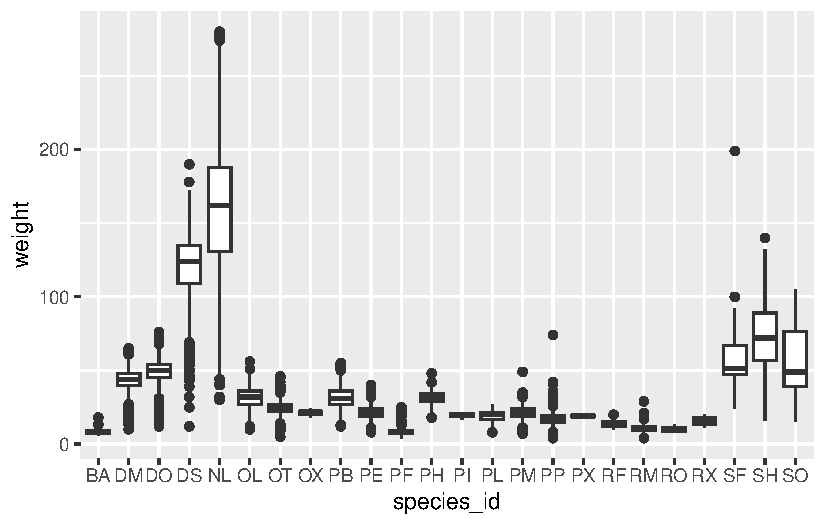
\includegraphics{src/r-basics_files/figure-pdf/unnamed-chunk-44-1.pdf}

\begin{Shaded}
\begin{Highlighting}[]
\CommentTok{\# add transparency}
\NormalTok{surveys\_plot }\SpecialCharTok{+} \FunctionTok{geom\_point}\NormalTok{(}\AttributeTok{alpha =} \FloatTok{0.1}\NormalTok{)}
\end{Highlighting}
\end{Shaded}

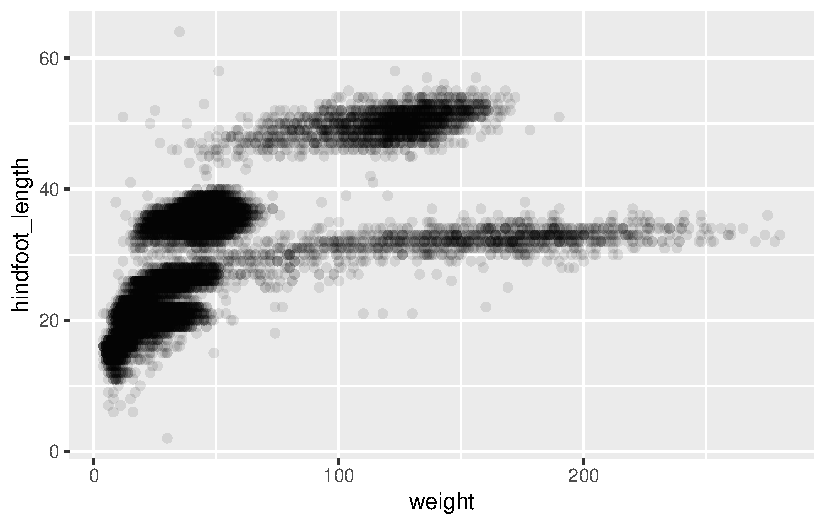
\includegraphics{src/r-basics_files/figure-pdf/unnamed-chunk-44-2.pdf}

\begin{Shaded}
\begin{Highlighting}[]
\CommentTok{\# color if not used in binding}
\NormalTok{surveys\_plot }\SpecialCharTok{+} \FunctionTok{geom\_point}\NormalTok{(}\AttributeTok{alpha =} \FloatTok{0.1}\NormalTok{, }\AttributeTok{color =} \StringTok{"black"}\NormalTok{)}
\end{Highlighting}
\end{Shaded}

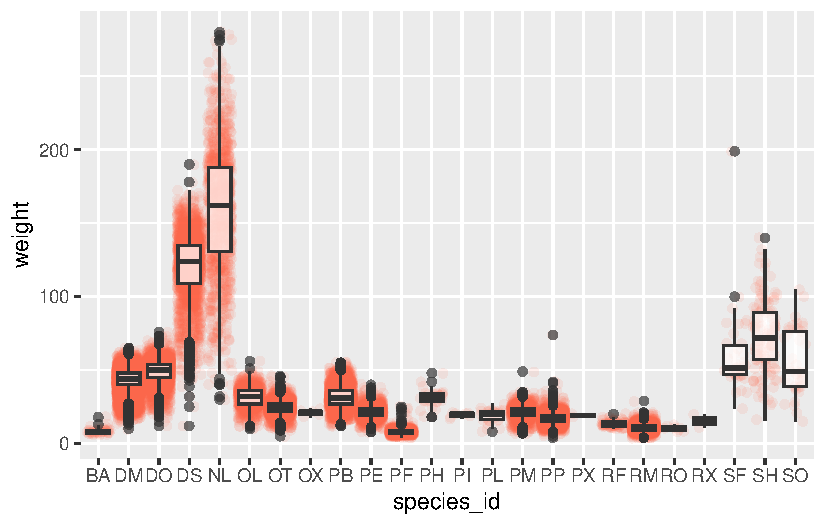
\includegraphics{src/r-basics_files/figure-pdf/unnamed-chunk-44-3.pdf}

\begin{Shaded}
\begin{Highlighting}[]
\CommentTok{\# add color if not used in binding}
\NormalTok{surveys\_plot }\SpecialCharTok{+} \FunctionTok{geom\_point}\NormalTok{(}\AttributeTok{alpha =} \FloatTok{0.1}\NormalTok{, }\FunctionTok{aes}\NormalTok{(}\AttributeTok{color =}\NormalTok{ species\_id))}
\end{Highlighting}
\end{Shaded}

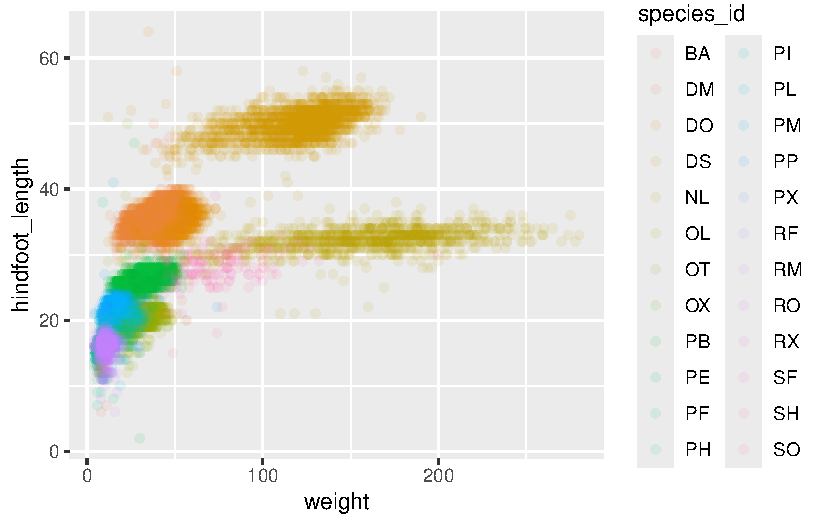
\includegraphics{src/r-basics_files/figure-pdf/unnamed-chunk-44-4.pdf}

\begin{Shaded}
\begin{Highlighting}[]
\CommentTok{\# make the color blend by introducing small random variation in points locations}
\CommentTok{\# used when having small data sets}
\NormalTok{surveys\_plot }\SpecialCharTok{+} \FunctionTok{geom\_jitter}\NormalTok{(}\AttributeTok{alpha =} \FloatTok{0.1}\NormalTok{)}
\end{Highlighting}
\end{Shaded}

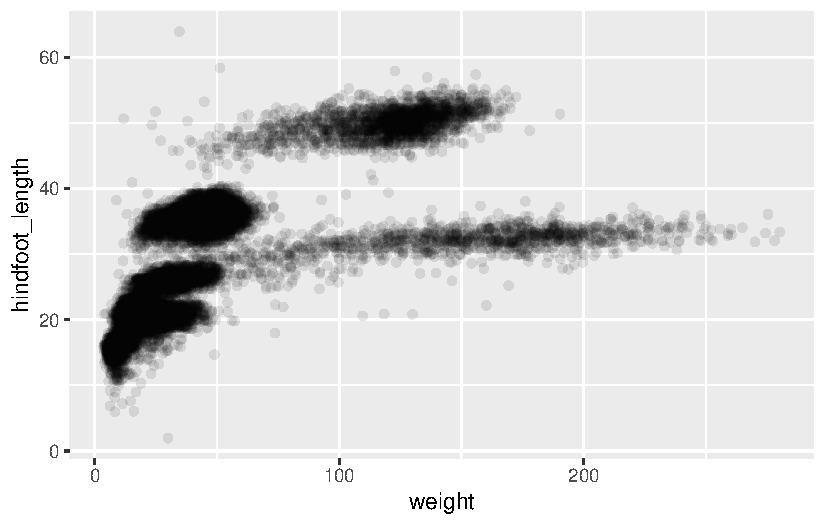
\includegraphics{src/r-basics_files/figure-pdf/unnamed-chunk-44-5.pdf}

\subsection{Boxplot}\label{boxplot}

\begin{Shaded}
\begin{Highlighting}[]
\NormalTok{surveys\_plot }\OtherTok{\textless{}{-}} \FunctionTok{ggplot}\NormalTok{(}\AttributeTok{data =}\NormalTok{ survey\_complete, }
    \AttributeTok{mapping =} \FunctionTok{aes}\NormalTok{(}\AttributeTok{x =}\NormalTok{ species\_id, }\AttributeTok{y =}\NormalTok{ weight))}

\NormalTok{surveys\_plot }\SpecialCharTok{+} \FunctionTok{geom\_boxplot}\NormalTok{()}
\end{Highlighting}
\end{Shaded}

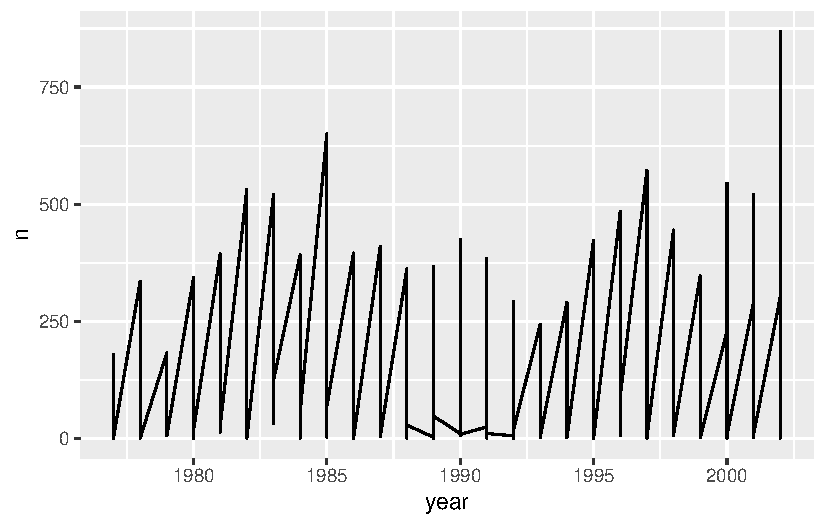
\includegraphics{src/r-basics_files/figure-pdf/unnamed-chunk-45-1.pdf}

\begin{Shaded}
\begin{Highlighting}[]
\CommentTok{\# show data}
\NormalTok{surveys\_plot }\SpecialCharTok{+} \FunctionTok{geom\_boxplot}\NormalTok{(}\AttributeTok{alpha =} \FloatTok{0.5}\NormalTok{) }\SpecialCharTok{+} 
    \FunctionTok{geom\_jitter}\NormalTok{(}\AttributeTok{alpha =} \FloatTok{0.1}\NormalTok{, }\AttributeTok{color =} \StringTok{"tomato"}\NormalTok{)}
\end{Highlighting}
\end{Shaded}

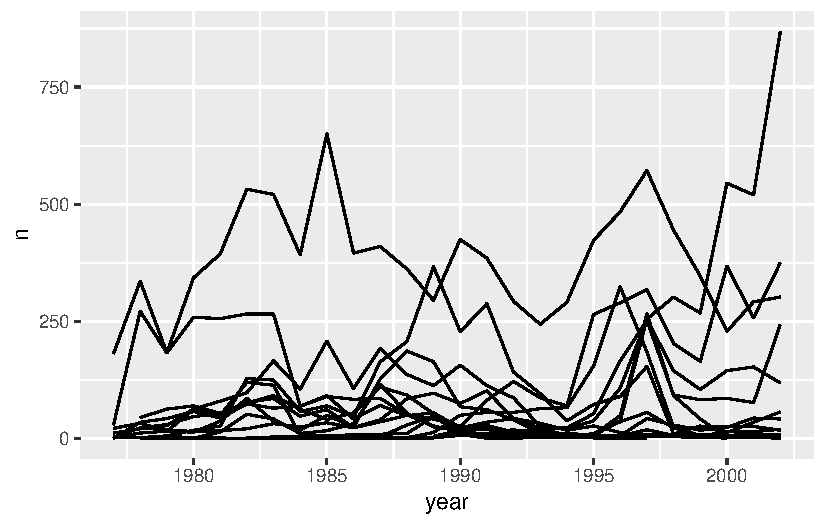
\includegraphics{src/r-basics_files/figure-pdf/unnamed-chunk-45-2.pdf}

\begin{Shaded}
\begin{Highlighting}[]
\CommentTok{\# bring boxplot layer in front}
\NormalTok{surveys\_plot }\SpecialCharTok{+} \FunctionTok{geom\_jitter}\NormalTok{(}\AttributeTok{alpha =} \FloatTok{0.1}\NormalTok{, }\AttributeTok{color =} \StringTok{"tomato"}\NormalTok{) }\SpecialCharTok{+}
    \FunctionTok{geom\_boxplot}\NormalTok{(}\AttributeTok{alpha =} \FloatTok{0.7}\NormalTok{)}
\end{Highlighting}
\end{Shaded}

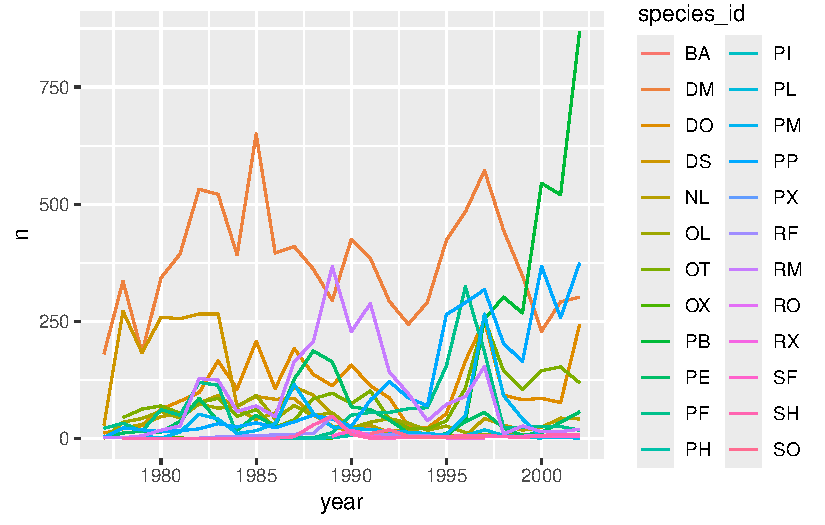
\includegraphics{src/r-basics_files/figure-pdf/unnamed-chunk-45-3.pdf}

\subsection{Time series data}\label{time-series-data}

\begin{Shaded}
\begin{Highlighting}[]
\CommentTok{\# create appropriate dataset}
\NormalTok{yearly\_count }\OtherTok{\textless{}{-}}\NormalTok{ survey\_complete }\SpecialCharTok{\%\textgreater{}\%}
    \FunctionTok{count}\NormalTok{(year, species\_id)}

\NormalTok{surveys\_plot }\OtherTok{\textless{}{-}} \FunctionTok{ggplot}\NormalTok{(}\AttributeTok{data =}\NormalTok{ yearly\_count, }
    \AttributeTok{mapping =} \FunctionTok{aes}\NormalTok{(}\AttributeTok{x =}\NormalTok{ year, }\AttributeTok{y =}\NormalTok{ n))}

\NormalTok{surveys\_plot }\SpecialCharTok{+} \FunctionTok{geom\_line}\NormalTok{()}
\end{Highlighting}
\end{Shaded}

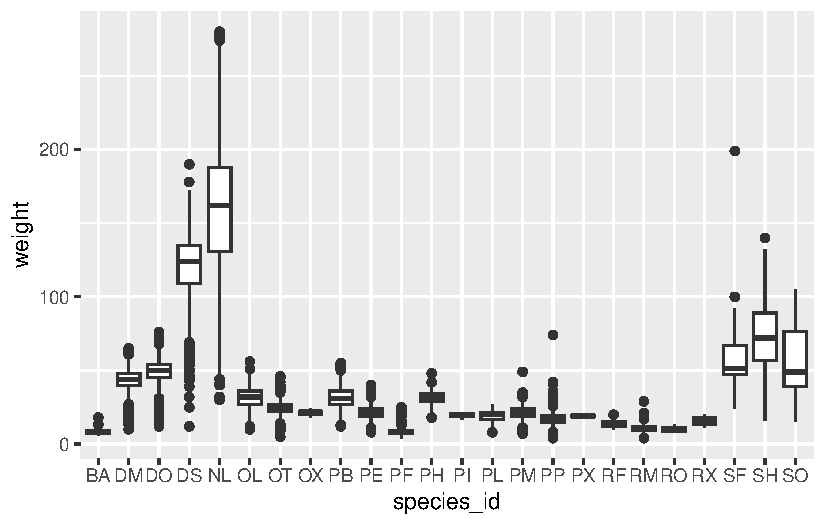
\includegraphics{src/r-basics_files/figure-pdf/unnamed-chunk-46-1.pdf}

\begin{Shaded}
\begin{Highlighting}[]
\CommentTok{\# make it more meaningful by breaking it by category}
\NormalTok{surveys\_plot }\SpecialCharTok{+} \FunctionTok{geom\_line}\NormalTok{(}\FunctionTok{aes}\NormalTok{(}\AttributeTok{group =}\NormalTok{ species\_id))}
\end{Highlighting}
\end{Shaded}

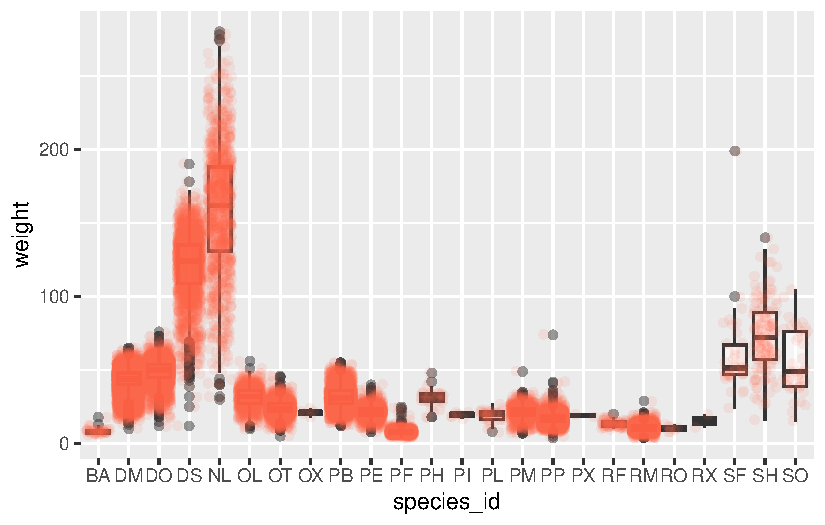
\includegraphics{src/r-basics_files/figure-pdf/unnamed-chunk-46-2.pdf}

\begin{Shaded}
\begin{Highlighting}[]
\CommentTok{\# make it more colorful}
\NormalTok{surveys\_plot }\SpecialCharTok{+} \FunctionTok{geom\_line}\NormalTok{(}\FunctionTok{aes}\NormalTok{(}\AttributeTok{color =}\NormalTok{ species\_id))}
\end{Highlighting}
\end{Shaded}

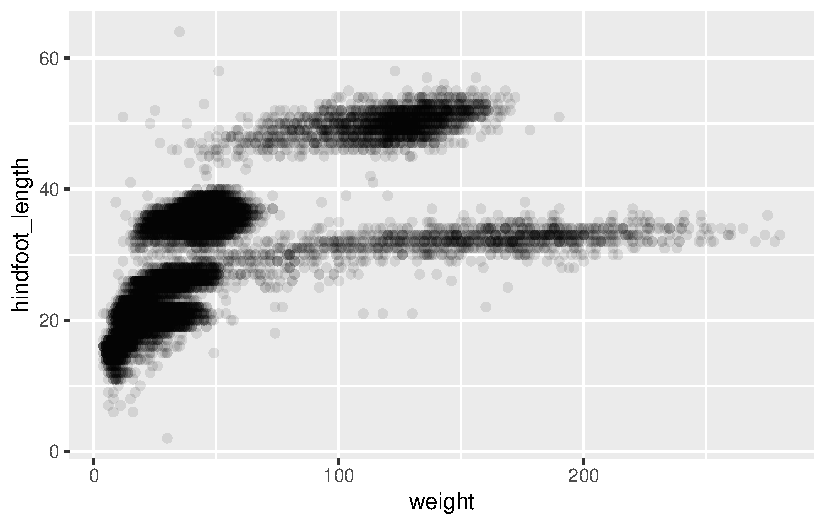
\includegraphics{src/r-basics_files/figure-pdf/unnamed-chunk-46-3.pdf}

\begin{Shaded}
\begin{Highlighting}[]
\CommentTok{\# split into multiple plots}
\NormalTok{surveys\_plot }\SpecialCharTok{+} \FunctionTok{geom\_line}\NormalTok{() }\SpecialCharTok{+} \FunctionTok{facet\_wrap}\NormalTok{(}\SpecialCharTok{\textasciitilde{}}\NormalTok{ species\_id)}
\end{Highlighting}
\end{Shaded}

\begin{verbatim}
`geom_line()`: Each group consists of only one observation.
i Do you need to adjust the group aesthetic?
\end{verbatim}

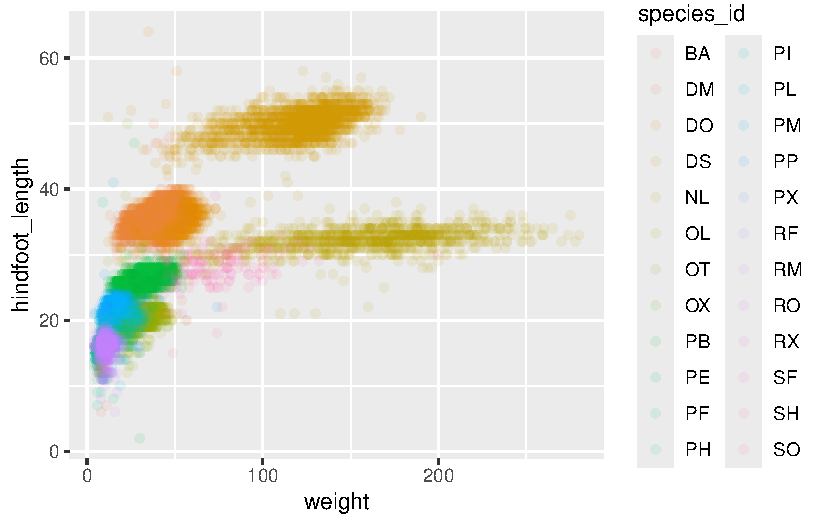
\includegraphics{src/r-basics_files/figure-pdf/unnamed-chunk-46-4.pdf}

\begin{Shaded}
\begin{Highlighting}[]
\CommentTok{\# split the line in each plot by sex}
\NormalTok{yearly\_sex\_counts }\OtherTok{\textless{}{-}}\NormalTok{ survey\_complete }\SpecialCharTok{\%\textgreater{}\%}
    \FunctionTok{count}\NormalTok{(year, species\_id, sex)}

\NormalTok{surveys\_plot }\OtherTok{\textless{}{-}} \FunctionTok{ggplot}\NormalTok{(}\AttributeTok{data =}\NormalTok{ yearly\_sex\_counts, }
    \AttributeTok{mapping =} \FunctionTok{aes}\NormalTok{(}\AttributeTok{x =}\NormalTok{ year, }\AttributeTok{y =}\NormalTok{ n))}

\NormalTok{surveys\_plot }\SpecialCharTok{+} \FunctionTok{geom\_line}\NormalTok{(}\FunctionTok{aes}\NormalTok{(}\AttributeTok{color =}\NormalTok{ sex)) }\SpecialCharTok{+}
    \FunctionTok{facet\_wrap}\NormalTok{(}\SpecialCharTok{\textasciitilde{}}\NormalTok{ species\_id)}
\end{Highlighting}
\end{Shaded}

\begin{verbatim}
`geom_line()`: Each group consists of only one observation.
i Do you need to adjust the group aesthetic?
\end{verbatim}

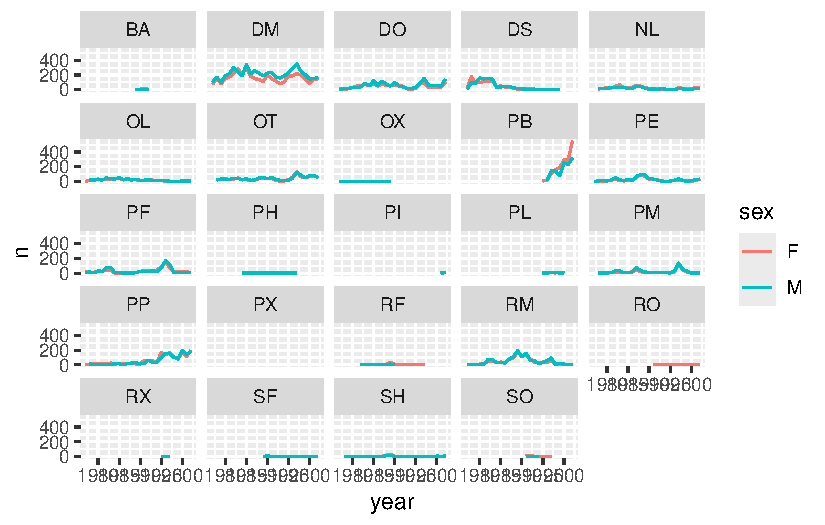
\includegraphics{src/r-basics_files/figure-pdf/unnamed-chunk-46-5.pdf}

\begin{Shaded}
\begin{Highlighting}[]
\CommentTok{\# remove background}
\NormalTok{surveys\_plot }\SpecialCharTok{+} \FunctionTok{geom\_line}\NormalTok{(}\FunctionTok{aes}\NormalTok{(}\AttributeTok{color =}\NormalTok{ sex)) }\SpecialCharTok{+}
    \FunctionTok{facet\_wrap}\NormalTok{(}\SpecialCharTok{\textasciitilde{}}\NormalTok{ species\_id) }\SpecialCharTok{+}
    \FunctionTok{theme\_bw}\NormalTok{() }\SpecialCharTok{+}
    \FunctionTok{theme}\NormalTok{(}\AttributeTok{panel.grid =} \FunctionTok{element\_blank}\NormalTok{())}
\end{Highlighting}
\end{Shaded}

\begin{verbatim}
`geom_line()`: Each group consists of only one observation.
i Do you need to adjust the group aesthetic?
\end{verbatim}

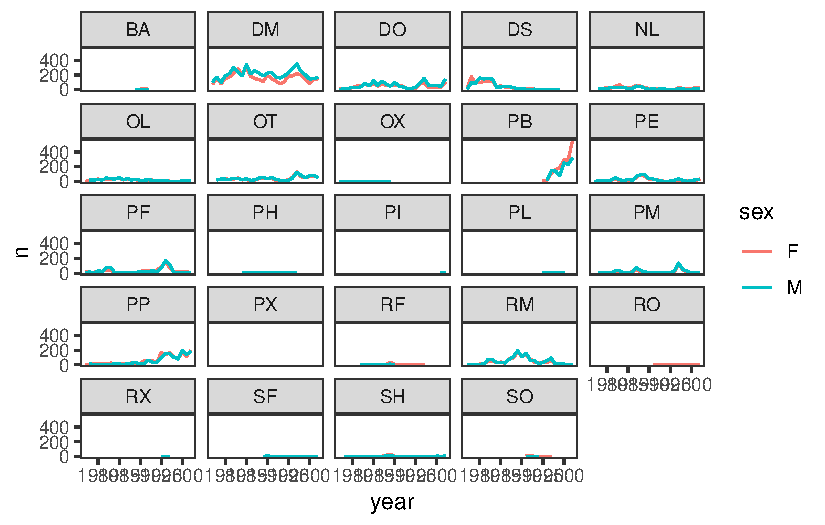
\includegraphics{src/r-basics_files/figure-pdf/unnamed-chunk-46-6.pdf}

\section{References}\label{references}

\begin{itemize}
\tightlist
\item
  OU Software Carpentry Workshop (check other workshops
  \href{https://libraries.ou.edu/content/software-and-data-carpentry}{here})

  \begin{itemize}
  \tightlist
  \item
    \href{https://oulib-swc.github.io/2019-05-15-ou-swc/}{Main Tutorial}
  \item
    \href{https://datacarpentry.org/R-ecology-lesson/index.html}{Data
    Carpentry with R}
  \item
    \href{https://swcarpentry.github.io/r-novice-gapminder/}{Software
    Carpentry with R}
  \item
    \href{https://pad.carpentries.org/2019-05-15-ou-swc}{Etherpad}
  \item
    \href{https://docs.google.com/document/d/1aJq_X1uhaNkUj7qdZEzOcpc2Pky7eZPy76yqs0UkfrQ/edit}{Google
    Doc}
  \end{itemize}
\item
  \href{https://rawcdn.githack.com/allisonhorst/data-vis/fc107e063f50ef8695b0a75ed73d74720aca2c65/data_vis_np.html}{Intro
  to ggplot} by \href{https://github.com/allisonhorst}{Allison Horst}
\item
  \href{https://r4ds.had.co.nz/}{R for Data Science book by Garrett
  Grolemund and Hadley Wickham}
\item
  \href{http://journals.plos.org/plosbiology/article?id=10.1371/journal.pbio.1001745}{Best
  Practices for Scientific Computing paper}
\end{itemize}

\part{Quarto}

\chapter{Quarto}\label{quarto-1}

\section{Render \& Review}\label{render-review}

\begin{enumerate}
\def\labelenumi{\arabic{enumi}.}
\tightlist
\item
  VSCode/RStudio -\textgreater{} \emph{Render} button
\item
  Terminal -\textgreater{} \texttt{quarto\ preview}
\item
  Terminal -\textgreater{} \texttt{quarto\ preview\ help}
\end{enumerate}

\section{Render w/o Review}\label{render-wo-review}

\begin{enumerate}
\def\labelenumi{\arabic{enumi}.}
\tightlist
\item
  Terminal -\textgreater{} \texttt{quarto\ render}
\item
  Terminal -\textgreater{} \texttt{quarto\ render\ help}
\end{enumerate}

\section{References}\label{references-1}

\begin{itemize}
\tightlist
\item
  \href{https://quarto.org/docs/reference/}{Quarto Reference}
\end{itemize}

\part{Practice}

\chapter{Topic Modeling, R}\label{topic-modeling-r}

\chapter{Introduction}\label{introduction}

An attempt to understand Sherlock Holmes short stories found in
Adventures of Sherlock Holmes book by Arthur Conan Doyle. After
inspecting the table of content, the book seems to have 12 stories, one
story per chapter. The analysis is inspired by
\href{https://juliasilge.com/}{Julia Silge}'s YouTube video
\href{https://www.youtube.com/watch?v=evTuL-RcRpc&t=321s}{Topic modeling
with R and tidy data principles}

\chapter{Download Book}\label{download-book}

\begin{Shaded}
\begin{Highlighting}[]
\FunctionTok{library}\NormalTok{(gutenbergr)  }\CommentTok{\# download books from Project Gutenberg using book ID}
\FunctionTok{library}\NormalTok{(tidyverse)}
\end{Highlighting}
\end{Shaded}

\begin{verbatim}
-- Attaching core tidyverse packages ------------------------ tidyverse 2.0.0 --
v dplyr     1.1.4     v readr     2.1.5
v forcats   1.0.0     v stringr   1.5.1
v ggplot2   3.5.1     v tibble    3.2.1
v lubridate 1.9.3     v tidyr     1.3.1
v purrr     1.0.2     
-- Conflicts ------------------------------------------ tidyverse_conflicts() --
x dplyr::filter() masks stats::filter()
x dplyr::lag()    masks stats::lag()
i Use the conflicted package (<http://conflicted.r-lib.org/>) to force all conflicts to become errors
\end{verbatim}

\begin{Shaded}
\begin{Highlighting}[]
\FunctionTok{library}\NormalTok{(tidytext)}

\CommentTok{\# Download the book, each line of the book is read into a seperate row}
\NormalTok{sherlock\_raw }\OtherTok{\textless{}{-}} \FunctionTok{gutenberg\_download}\NormalTok{(}\DecValTok{48320}\NormalTok{)}
\end{Highlighting}
\end{Shaded}

\begin{verbatim}
Determining mirror for Project Gutenberg from https://www.gutenberg.org/robot/harvest
Using mirror http://aleph.gutenberg.org
\end{verbatim}

\begin{Shaded}
\begin{Highlighting}[]
\FunctionTok{dim}\NormalTok{(sherlock\_raw)}
\end{Highlighting}
\end{Shaded}

\begin{verbatim}
[1] 12350     2
\end{verbatim}

\begin{Shaded}
\begin{Highlighting}[]
\FunctionTok{head}\NormalTok{(sherlock\_raw)}
\end{Highlighting}
\end{Shaded}

\begin{verbatim}
# A tibble: 6 x 2
  gutenberg_id text                           
         <int> <chr>                          
1        48320 "ADVENTURES OF SHERLOCK HOLMES"
2        48320 ""                             
3        48320 ""                             
4        48320 ""                             
5        48320 ""                             
6        48320 "[Illustration:"               
\end{verbatim}

\begin{Shaded}
\begin{Highlighting}[]
\FunctionTok{tail}\NormalTok{(sherlock\_raw)}
\end{Highlighting}
\end{Shaded}

\begin{verbatim}
# A tibble: 6 x 2
  gutenberg_id text                                                  
         <int> <chr>                                                 
1        48320 "  boisterious fashion, and on the whole _changed to_"
2        48320 "  boisterous fashion, and on the whole"              
3        48320 ""                                                    
4        48320 "  Page 297"                                          
5        48320 "  wrapt in the peaceful beauty _changed to_"         
6        48320 "  rapt in the peaceful beauty"                       
\end{verbatim}

\chapter{Wrangle: Label Stories}\label{wrangle-label-stories}

\begin{Shaded}
\begin{Highlighting}[]
\NormalTok{sherlock }\OtherTok{\textless{}{-}}\NormalTok{ sherlock\_raw }\SpecialCharTok{\%\textgreater{}\%} 
  
  \CommentTok{\# determine start of each story/chapter}
  \FunctionTok{mutate}\NormalTok{(}\AttributeTok{story =} \FunctionTok{ifelse}\NormalTok{(}\FunctionTok{str\_detect}\NormalTok{(text, }\StringTok{"\^{}(A SCANDAL IN BOHEMIA|THE RED{-}HEADED LEAGUE|A CASE OF IDENTITY|THE BOSCOMBE VALLEY MYSTERY|THE FIVE ORANGE PIPS|THE MAN WITH THE TWISTED LIP|THE ADVENTURE OF THE BLUE CARBUNCLE|THE ADVENTURE OF THE SPECKLED BAND|THE ADVENTURE OF THE ENGINEER’S THUMB|THE ADVENTURE OF THE NOBLE BACHELOR|THE ADVENTURE OF THE BERYL CORONET|THE ADVENTURE OF THE COPPER BEECHES)$"}\NormalTok{), text, }\ConstantTok{NA}\NormalTok{)) }\SpecialCharTok{\%\textgreater{}\%}
  
  \CommentTok{\# determine lines belonging to each story/chapter by}
  \CommentTok{\# filling down the N/A rows of story column}
  \FunctionTok{fill}\NormalTok{(story) }\SpecialCharTok{\%\textgreater{}\%}
  
  \CommentTok{\# remove the part that does not belong to any story/chapter,}
  \CommentTok{\# i.e, the introduction}
  \FunctionTok{filter}\NormalTok{(}\SpecialCharTok{!}\FunctionTok{is.na}\NormalTok{(story)) }\SpecialCharTok{\%\textgreater{}\%}
  
  \CommentTok{\# convert story column to factor}
  \FunctionTok{mutate}\NormalTok{(}\AttributeTok{story =} \FunctionTok{factor}\NormalTok{(story))}
\end{Highlighting}
\end{Shaded}

\chapter{Wrangle: Put in Tidy Format}\label{wrangle-put-in-tidy-format}

The row of \texttt{text} column contains multiple words/tokens. We want
to put each word/token of each \texttt{text} row into a separate row.
This makes the dataframe follows the tidy format and hence makes it easy
to process.

\begin{Shaded}
\begin{Highlighting}[]
\NormalTok{tidy\_sherlock }\OtherTok{\textless{}{-}}\NormalTok{ sherlock }\SpecialCharTok{\%\textgreater{}\%}
  
  \CommentTok{\# number the rows}
  \FunctionTok{mutate}\NormalTok{(}\AttributeTok{line =} \FunctionTok{row\_number}\NormalTok{()) }\SpecialCharTok{\%\textgreater{}\%} 
  
  \CommentTok{\# break the text column into multiple row where each row contain one token}
  \FunctionTok{unnest\_tokens}\NormalTok{(word, text) }\SpecialCharTok{\%\textgreater{}\%} 
  
  \CommentTok{\# remove the stopwords{-}{-}the rows where the word column is a stopword}
  \FunctionTok{anti\_join}\NormalTok{(stop\_words) }\SpecialCharTok{\%\textgreater{}\%} 
  
  \CommentTok{\# remove holmes rows which might affect our topic models}
  \FunctionTok{filter}\NormalTok{(word }\SpecialCharTok{!=} \StringTok{"holmes"}\NormalTok{)}
\end{Highlighting}
\end{Shaded}

\begin{verbatim}
Joining with `by = join_by(word)`
\end{verbatim}

\chapter{Explore tf-idf}\label{explore-tf-idf}

\begin{itemize}
\tightlist
\item
  To see which words are important in each story/chapter, i.e.,the words
  that appears many times in that story but few or none in the other
  stories.
\item
  tf-idf (term frequency-inverse document frequency) is a great
  exploratory tool before starting with topic modeling
\end{itemize}

\begin{Shaded}
\begin{Highlighting}[]
\FunctionTok{library}\NormalTok{(ggplot2)}

\NormalTok{tidy\_sherlock }\SpecialCharTok{\%\textgreater{}\%} 
  
  \CommentTok{\# count number of occurrence of words in stories}
  \FunctionTok{count}\NormalTok{(story, word, }\AttributeTok{sort =} \ConstantTok{TRUE}\NormalTok{) }\SpecialCharTok{\%\textgreater{}\%} 
  
  \CommentTok{\# compute and add tf, idf, and tf\_idf values for words}
  \FunctionTok{bind\_tf\_idf}\NormalTok{(word, story, n) }\SpecialCharTok{\%\textgreater{}\%} 
  
  \CommentTok{\# group by story}
  \FunctionTok{group\_by}\NormalTok{(story) }\SpecialCharTok{\%\textgreater{}\%} 
  
  \CommentTok{\# take top 10 words of each story with highest tf\_idf (last column)}
  \FunctionTok{top\_n}\NormalTok{(}\DecValTok{10}\NormalTok{) }\SpecialCharTok{\%\textgreater{}\%} 
  
  \CommentTok{\# unpack}
  \FunctionTok{ungroup}\NormalTok{() }\SpecialCharTok{\%\textgreater{}\%} 
  
  \CommentTok{\# turn words into factors and order them based on their tf\_idf values}
  \CommentTok{\# }\AlertTok{NOTE}\CommentTok{: This will not affect order the dataframe rows which is can be}
  \CommentTok{\#   done via the arrange function}
  \CommentTok{\# }\AlertTok{NOTE}\CommentTok{: Recording the word column this way is for ggplot to visualize them}
  \CommentTok{\#   as desired from top tf\_idf to lowest}
  \FunctionTok{mutate}\NormalTok{(}\AttributeTok{word =} \FunctionTok{reorder}\NormalTok{(word, tf\_idf)) }\SpecialCharTok{\%\textgreater{}\%} 
  
  \CommentTok{\# plot}
  \FunctionTok{ggplot}\NormalTok{(}\FunctionTok{aes}\NormalTok{(word, tf\_idf, }\AttributeTok{fill =}\NormalTok{ story)) }\SpecialCharTok{+}
  \FunctionTok{geom\_col}\NormalTok{(}\AttributeTok{show.legend =} \ConstantTok{FALSE}\NormalTok{) }\SpecialCharTok{+}
  \FunctionTok{facet\_wrap}\NormalTok{(}\SpecialCharTok{\textasciitilde{}}\NormalTok{story, }\AttributeTok{scales =} \StringTok{"free"}\NormalTok{, }\AttributeTok{ncol =} \DecValTok{3}\NormalTok{) }\SpecialCharTok{+}
  \FunctionTok{theme}\NormalTok{(}\AttributeTok{strip.text.x =} \FunctionTok{element\_text}\NormalTok{(}\AttributeTok{size =} \DecValTok{5}\NormalTok{)) }\SpecialCharTok{+}
  \FunctionTok{coord\_flip}\NormalTok{()}
\end{Highlighting}
\end{Shaded}

\begin{verbatim}
Selecting by tf_idf
\end{verbatim}


\includegraphics{src/topic-modeling-r_files/figure-pdf/unnamed-chunk-4-1.pdf}

\chapter{Implement Topic Modeling}\label{implement-topic-modeling}

Training the model for the topics

\begin{Shaded}
\begin{Highlighting}[]
\FunctionTok{library}\NormalTok{(stm)        }\CommentTok{\# for do topic modeling}
\end{Highlighting}
\end{Shaded}

\begin{verbatim}
stm v1.3.7 successfully loaded. See ?stm for help. 
 Papers, resources, and other materials at structuraltopicmodel.com
\end{verbatim}

\begin{Shaded}
\begin{Highlighting}[]
\FunctionTok{library}\NormalTok{(quanteda)   }\CommentTok{\# great text mining, will be used to structure the input}
\end{Highlighting}
\end{Shaded}

\begin{verbatim}
Package version: 4.0.2
Unicode version: 15.1
ICU version: 74.1
\end{verbatim}

\begin{verbatim}
Parallel computing: 8 of 8 threads used.
\end{verbatim}

\begin{verbatim}
See https://quanteda.io for tutorials and examples.
\end{verbatim}

\begin{Shaded}
\begin{Highlighting}[]
                    \CommentTok{\#   to stm}

\CommentTok{\# Convert from tidy form to quanteda form (document x term matrix)}
\NormalTok{sherlock\_stm }\OtherTok{\textless{}{-}}\NormalTok{ tidy\_sherlock }\SpecialCharTok{\%\textgreater{}\%} 
  \FunctionTok{count}\NormalTok{(story, word, }\AttributeTok{sort =} \ConstantTok{TRUE}\NormalTok{) }\SpecialCharTok{\%\textgreater{}\%} 
  \FunctionTok{cast\_dfm}\NormalTok{(story, word, n)}

\CommentTok{\# Train the model}
\NormalTok{topic\_model }\OtherTok{\textless{}{-}} \FunctionTok{stm}\NormalTok{(sherlock\_stm, }\AttributeTok{K=}\DecValTok{6}\NormalTok{, }\AttributeTok{init.type =} \StringTok{"Spectral"}\NormalTok{)}
\end{Highlighting}
\end{Shaded}

\begin{verbatim}
Beginning Spectral Initialization 
     Calculating the gram matrix...
     Finding anchor words...
    ......
     Recovering initialization...
    .............................................................................
Initialization complete.
............
Completed E-Step (0 seconds). 
Completed M-Step. 
Completing Iteration 1 (approx. per word bound = -7.785) 
............
Completed E-Step (0 seconds). 
Completed M-Step. 
Completing Iteration 2 (approx. per word bound = -7.593, relative change = 2.458e-02) 
............
Completed E-Step (0 seconds). 
Completed M-Step. 
Completing Iteration 3 (approx. per word bound = -7.481, relative change = 1.473e-02) 
............
Completed E-Step (0 seconds). 
Completed M-Step. 
Completing Iteration 4 (approx. per word bound = -7.455, relative change = 3.469e-03) 
............
Completed E-Step (0 seconds). 
Completed M-Step. 
Completing Iteration 5 (approx. per word bound = -7.450, relative change = 7.612e-04) 
Topic 1: st, simon, lord, day, lady 
 Topic 2: door, miss, house, rucastle, matter 
 Topic 3: hat, goose, stone, bird, geese 
 Topic 4: father, time, mccarthy, son, hand 
 Topic 5: house, time, night, door, heard 
 Topic 6: red, time, wilson, business, headed 
............
Completed E-Step (0 seconds). 
Completed M-Step. 
Completing Iteration 6 (approx. per word bound = -7.449, relative change = 1.233e-04) 
............
Completed E-Step (0 seconds). 
Completed M-Step. 
Completing Iteration 7 (approx. per word bound = -7.449, relative change = 1.168e-05) 
............
Completed E-Step (0 seconds). 
Completed M-Step. 
Model Converged 
\end{verbatim}

\begin{Shaded}
\begin{Highlighting}[]
\FunctionTok{summary}\NormalTok{(topic\_model)}
\end{Highlighting}
\end{Shaded}

\begin{verbatim}
A topic model with 6 topics, 12 documents and a 7709 word dictionary.
\end{verbatim}

\begin{verbatim}
Topic 1 Top Words:
     Highest Prob: st, simon, lord, day, lady, found, matter 
     FREX: simon, clair, neville, lascar, opium, doran, flora 
     Lift: aloysius, ceremony, doran, millar, 2_s, aberdeen, absurdly 
     Score: simon, st, clair, neville, _danseuse_, lestrade, doran 
Topic 2 Top Words:
     Highest Prob: door, miss, house, rucastle, matter, street, lady 
     FREX: rucastle, hosmer, hunter, angel, windibank, _changed, 1 
     Lift: advertised, angel, annoyance, brothers, employed, factor, fowler 
     Score: rucastle, hosmer, angel, windibank, hunter, type, 1 
Topic 3 Top Words:
     Highest Prob: hat, goose, stone, bird, geese, baker, sir 
     FREX: geese, horner, ryder, henry, peterson, salesman, countess 
     Lift: battered, bet, bred, brixton, cosmopolitan, covent, cream 
     Score: goose, geese, horner, _alias_, ryder, henry, peterson 
Topic 4 Top Words:
     Highest Prob: father, time, mccarthy, son, hand, lestrade, left 
     FREX: mccarthy, pool, boscombe, openshaw, pips, horsham, turner 
     Lift: bone, dundee, horsham, pondicherry, presumption, savannah, sundial 
     Score: mccarthy, pool, lestrade, boscombe, openshaw, _détour_, turner 
Topic 5 Top Words:
     Highest Prob: house, time, night, door, heard, hand, round 
     FREX: coronet, stoner, arthur, roylott, ventilator, gems, stoke 
     Lift: _absolute_, _all_, _en, 1100, 16a, 3d, 4000 
     Score: coronet, arthur, stoner, gems, 4000, roylott, ventilator 
Topic 6 Top Words:
     Highest Prob: red, time, wilson, business, headed, day, league 
     FREX: wilson, league, merryweather, jones, coburg, jabez, headed 
     Lift: daring, saturday, vincent, _employé_, _october, _partie, 17 
     Score: wilson, league, merryweather, _employé_, jones, headed, coburg 
\end{verbatim}

\chapter{Contribution of Words in
Topics}\label{contribution-of-words-in-topics}

Looking at which words contribute the most in each topic.

\begin{Shaded}
\begin{Highlighting}[]
\CommentTok{\# Extracting betas and putting them in a tidy format}
\NormalTok{tm\_beta }\OtherTok{\textless{}{-}} \FunctionTok{tidy}\NormalTok{(topic\_model)}

\CommentTok{\# Visualizing the top words contributing to each topic}
\NormalTok{tm\_beta }\SpecialCharTok{\%\textgreater{}\%} 
  \FunctionTok{group\_by}\NormalTok{(topic) }\SpecialCharTok{\%\textgreater{}\%} 
  \CommentTok{\# top 10 word in each topic with higest beta (last column)}
  \FunctionTok{top\_n}\NormalTok{(}\DecValTok{10}\NormalTok{) }\SpecialCharTok{\%\textgreater{}\%} 
  \FunctionTok{ungroup}\NormalTok{() }\SpecialCharTok{\%\textgreater{}\%} 
  \CommentTok{\# turn words into factors and order them based on their tf\_idf values}
  \CommentTok{\# }\AlertTok{NOTE}\CommentTok{: This will not affect order the dataframe rows which is can be}
  \CommentTok{\#   done via the arrange function}
  \CommentTok{\# }\AlertTok{NOTE}\CommentTok{: Recording the word column this way is for ggplot to visualize them}
  \CommentTok{\#   as desired from top tf\_idf to lowest}
  \FunctionTok{mutate}\NormalTok{(}\AttributeTok{term =} \FunctionTok{reorder}\NormalTok{(term, beta)) }\SpecialCharTok{\%\textgreater{}\%} 
  \FunctionTok{ggplot}\NormalTok{(}\FunctionTok{aes}\NormalTok{(term, beta, }\AttributeTok{fill =}\NormalTok{ topic)) }\SpecialCharTok{+}
  \FunctionTok{geom\_col}\NormalTok{(}\AttributeTok{show.legend =} \ConstantTok{FALSE}\NormalTok{) }\SpecialCharTok{+}
  \FunctionTok{facet\_wrap}\NormalTok{(}\SpecialCharTok{\textasciitilde{}}\NormalTok{topic, }\AttributeTok{scales =} \StringTok{"free"}\NormalTok{, }\AttributeTok{ncol =} \DecValTok{3}\NormalTok{) }\SpecialCharTok{+}
  \FunctionTok{coord\_flip}\NormalTok{()}
\end{Highlighting}
\end{Shaded}

\begin{verbatim}
Selecting by beta
\end{verbatim}


\includegraphics{src/topic-modeling-r_files/figure-pdf/unnamed-chunk-7-1.pdf}

\chapter{Distribution of Topics in
Stories}\label{distribution-of-topics-in-stories}

Looking at how the stories are associated with each topic and how strong
each association is.

\begin{Shaded}
\begin{Highlighting}[]
\CommentTok{\# Extracting gammas and putting them in a tidy format}
\NormalTok{tm\_gamma }\OtherTok{\textless{}{-}} \FunctionTok{tidy}\NormalTok{(topic\_model, }\AttributeTok{matrix =} \StringTok{"gamma"}\NormalTok{,}
                 \CommentTok{\# use the names of the stories instead of the default numbers}
                 \AttributeTok{document\_names =} \FunctionTok{rownames}\NormalTok{(sherlock\_stm))}


\CommentTok{\# Visualizing the number of stories belonging to each topics and the confidence}
\CommentTok{\#   of the belonging}
\NormalTok{tm\_gamma }\SpecialCharTok{\%\textgreater{}\%} 
  \FunctionTok{ggplot}\NormalTok{(}\FunctionTok{aes}\NormalTok{(gamma, }\AttributeTok{fill =} \FunctionTok{as.factor}\NormalTok{(topic))) }\SpecialCharTok{+}
  \FunctionTok{geom\_histogram}\NormalTok{(}\AttributeTok{show.legend =} \ConstantTok{FALSE}\NormalTok{) }\SpecialCharTok{+}
  \FunctionTok{facet\_wrap}\NormalTok{(}\SpecialCharTok{\textasciitilde{}}\NormalTok{topic, }\AttributeTok{ncol =} \DecValTok{3}\NormalTok{)}
\end{Highlighting}
\end{Shaded}

\begin{verbatim}
`stat_bin()` using `bins = 30`. Pick better value with `binwidth`.
\end{verbatim}

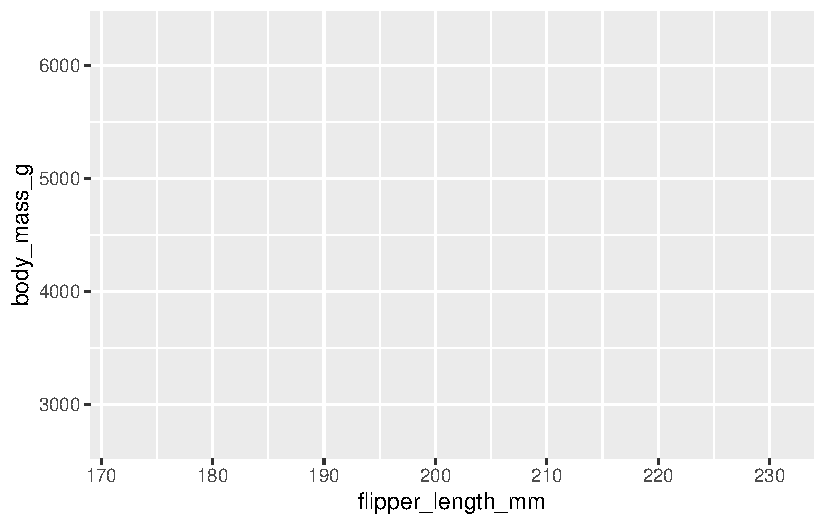
\includegraphics{src/topic-modeling-r_files/figure-pdf/unnamed-chunk-8-1.pdf}

\begin{Shaded}
\begin{Highlighting}[]
\CommentTok{\# Visualizing how much each topic appear in each story}
\NormalTok{tm\_gamma }\SpecialCharTok{\%\textgreater{}\%} 
  \FunctionTok{ggplot}\NormalTok{(}\FunctionTok{aes}\NormalTok{(topic, gamma, }\AttributeTok{fill =}\NormalTok{ document)) }\SpecialCharTok{+}
  \FunctionTok{geom\_col}\NormalTok{(}\AttributeTok{show.legend =} \ConstantTok{FALSE}\NormalTok{) }\SpecialCharTok{+}
  \FunctionTok{facet\_wrap}\NormalTok{(}\SpecialCharTok{\textasciitilde{}}\NormalTok{document, }\AttributeTok{scales =} \StringTok{"free"}\NormalTok{, }\AttributeTok{ncol =} \DecValTok{3}\NormalTok{) }\SpecialCharTok{+}
  \FunctionTok{theme}\NormalTok{(}\AttributeTok{strip.text.x =} \FunctionTok{element\_text}\NormalTok{(}\AttributeTok{size =} \DecValTok{5}\NormalTok{))}
\end{Highlighting}
\end{Shaded}

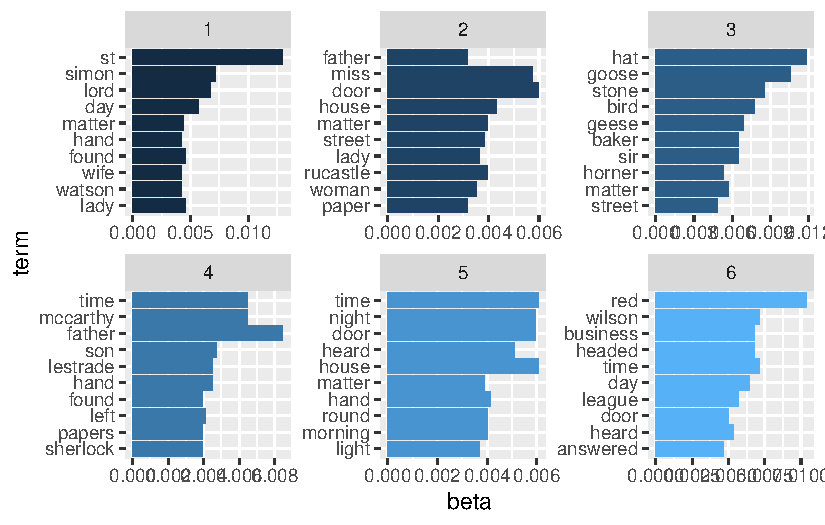
\includegraphics{src/topic-modeling-r_files/figure-pdf/unnamed-chunk-9-1.pdf}

The model did an excellent job strongly associating the stories into one
or more topics. This perfect association is rare in the world of topic
modeling. The reason behind this perfect association here could be due
to the small number of documents that we have.

\chapter{References}\label{references-2}

\begin{itemize}
\tightlist
\item
  Adventures of Sherlock Holmes book by Arthur Conan Doyle on
  \href{https://www.gutenberg.org/ebooks/48320}{Project Gutenberg}
\item
  \href{https://regex101.com/}{Regular Expressions 101}
\end{itemize}



\end{document}
